\documentclass[aspectratio=169]{beamer}
%\usetheme{Boadilla}
%\usetheme{default}
\usecolortheme{owl}
\usepackage{color}
\usepackage{fontawesome}
\usepackage{hyperref}
\hypersetup{
    colorlinks=true,
    linkcolor=blue,
    filecolor=magenta,      
    urlcolor=blue,
}

\urlstyle{same}


\title{\textbf{You've Been Hacked}}
\subtitle{An (Interactive) Course on Web Security\newline\vfill}
\author{\textbf{Paul Duplys}}
\institute[]{\faTwitter\hspace{0.1cm} @duplys \hspace{1cm} \faGithub\hspace{0.1cm} duplys \hspace{1cm} \faLinkedinSquare\hspace{0.1cm} linkedin.com/in/paulduplys/}
\date{}

\begin{document}

{
\usebackgroundtemplate{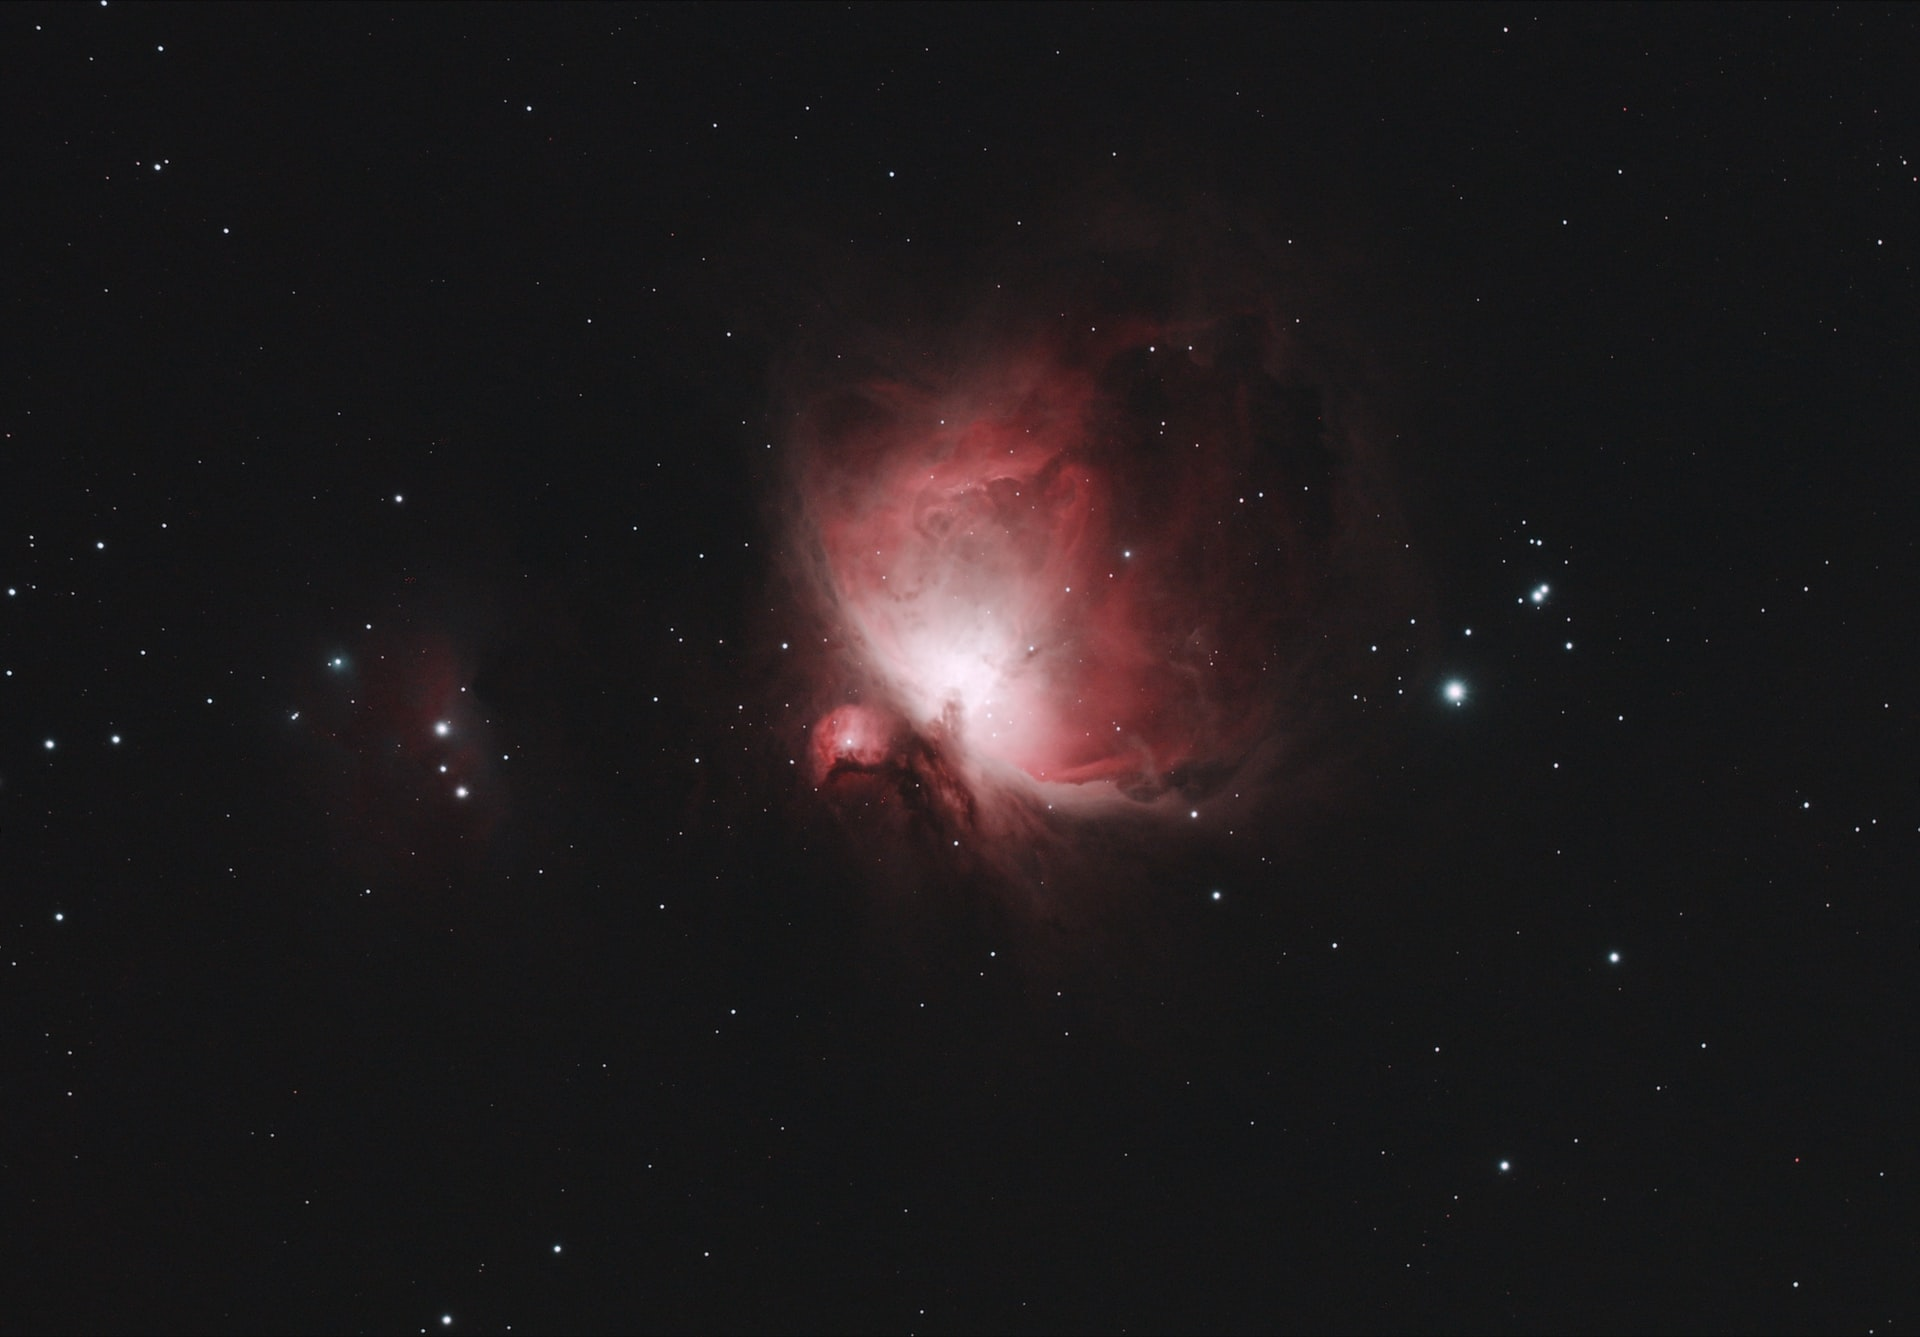
\includegraphics[width=\paperwidth]{./img/orion-nebula.jpg}}
\begin{frame}
    \titlepage
\end{frame}
}

\begin{frame}
    %\frametitle{Outline}
    \tableofcontents
\end{frame}

\section{0x0: Preliminaries}

{
\usebackgroundtemplate{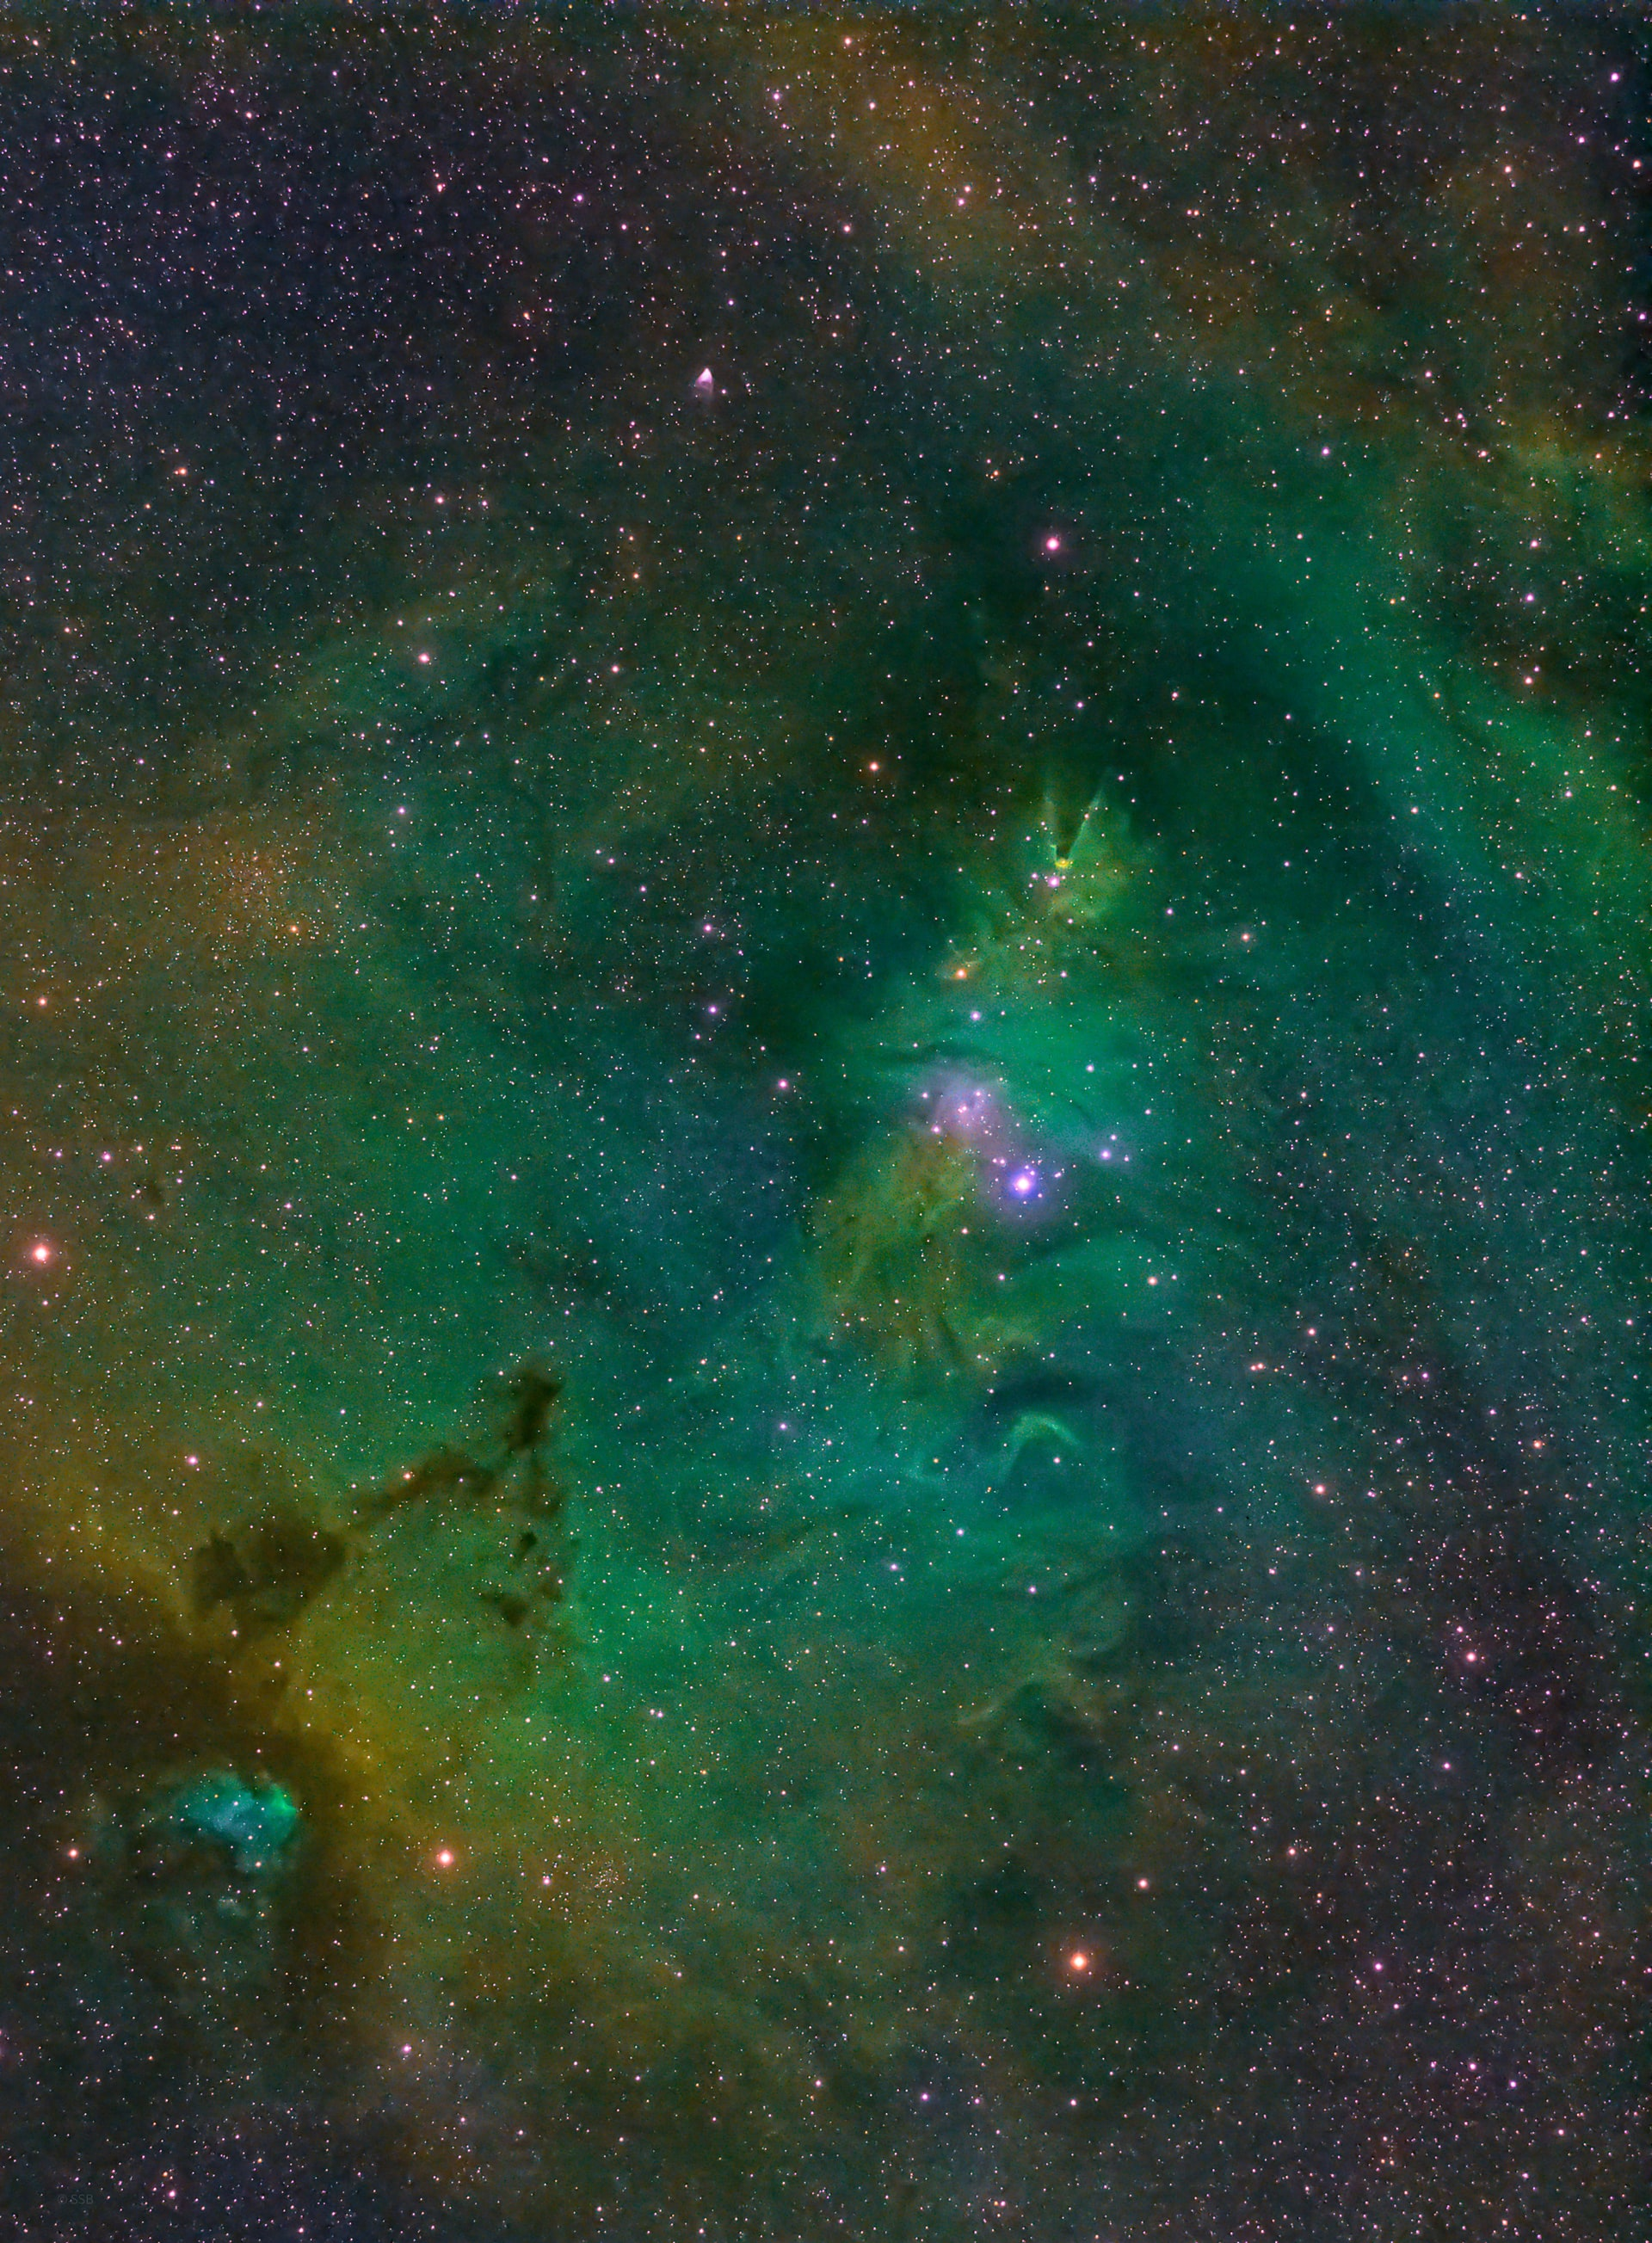
\includegraphics[width=\paperwidth]{./img/aldebaran.jpg}}
\begin{frame}
\huge{\textcolor{white}{\textbf{0x0: Preliminaries}}}
\end{frame}
}

\begin{frame}
    \frametitle{\texttt{whoami}}
    short intro/bio.
\end{frame}

\begin{frame}
    \frametitle{\texttt{man slides}}

    (Interactive) course on web security based on Carsten Eiler's book "You've Been Hacked".
    
    Who is the audience? How can I use the book? How can I explore the app?
\end{frame}

\begin{frame}
    \frametitle{\texttt{docker image ls}}
    Where are the instruction located for how to build the Docker files and use the repository?
\end{frame}

\section{0x1: Web Security 101}

{
\usebackgroundtemplate{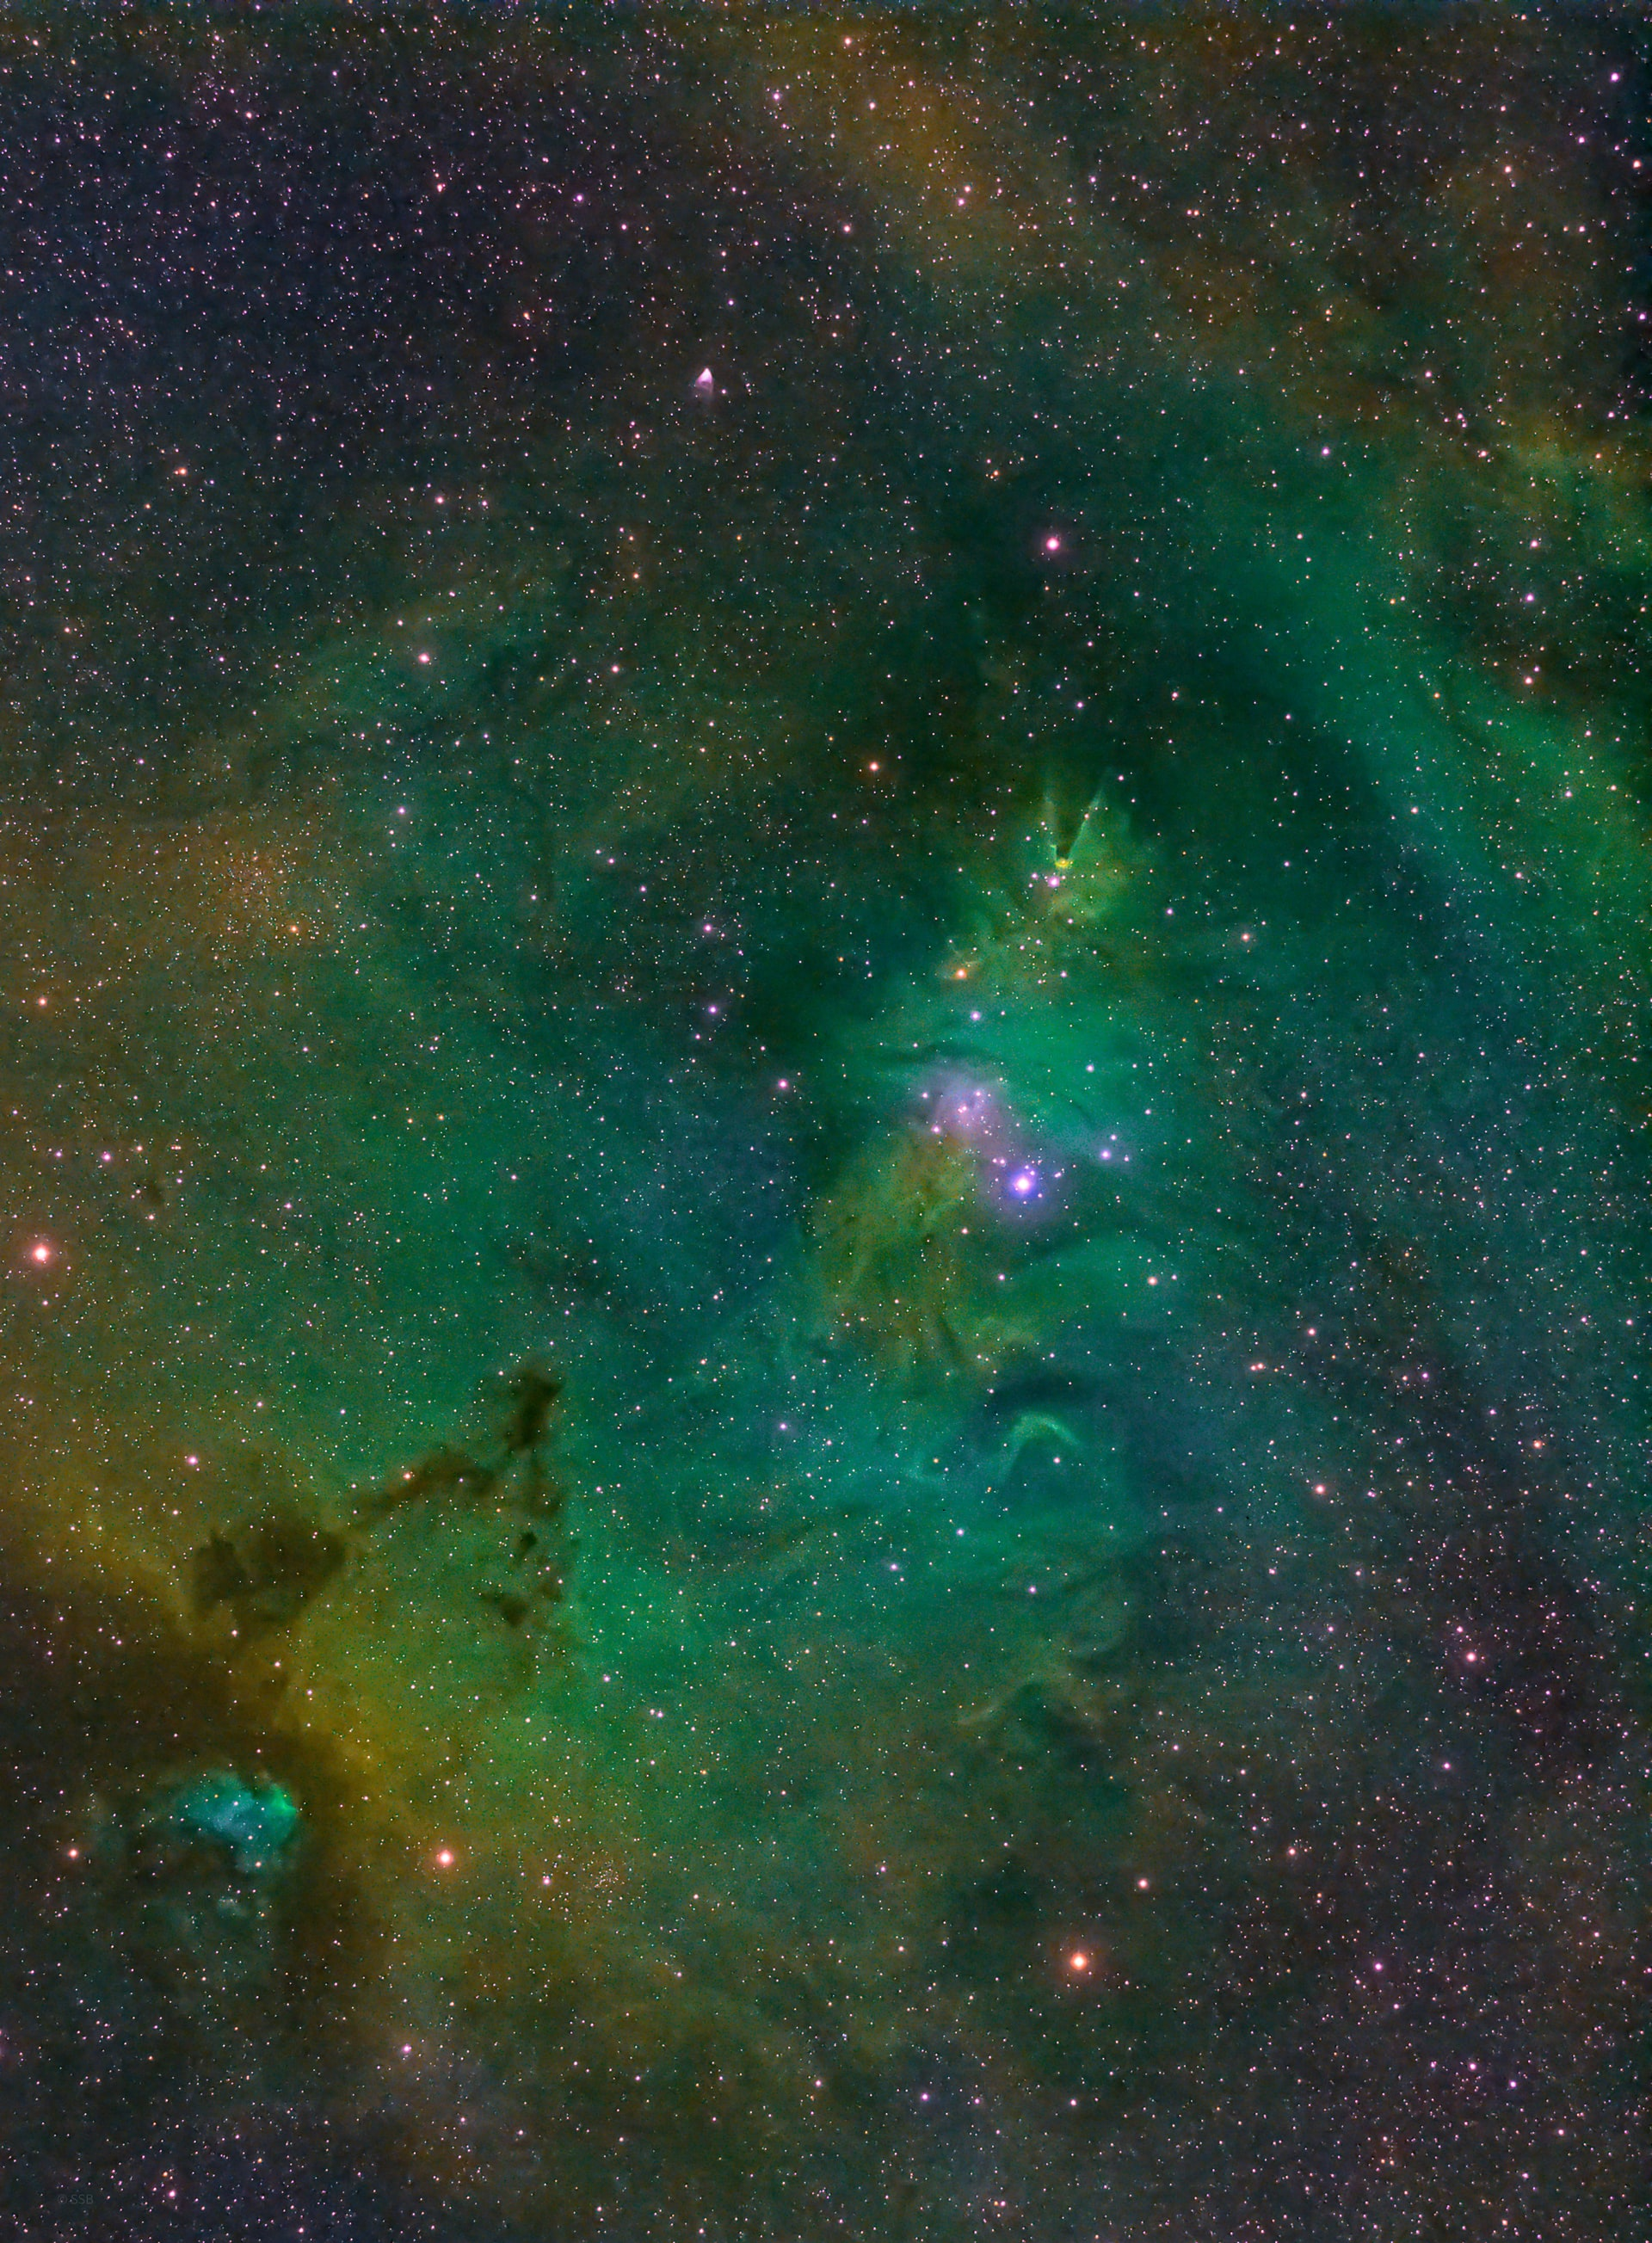
\includegraphics[width=\paperwidth]{./img/aldebaran.jpg}}
\begin{frame}
\huge{\textcolor{white}{\textbf{0x1: Web Security 101}}}
\end{frame}
}

\begin{frame}
    %\frametitle{How Do You Find Vulnerabilities in Web Applications?}
    In a nutshell, \textbf{to find vulnerabilities in your web application}, ...
    \begin{enumerate}
        \item ... test various values for parameters used by the web application and see what happens (conceptually similar to fuzzing)
        \item ... check web application code for bugs that may lead to security vulnerabilities (typically missing checks of input values or missing countermeasures against certain types of attacks)
    \end{enumerate}
\end{frame}

\begin{frame}
    %\frametitle{OWASP TOP 10}

    The \href{https://owasp.org/www-project-top-ten/}{Open Web Application Security Project (OWASP)} maintains a list of Top 10 vulnerabilities in web applications.

    \begin{center}
        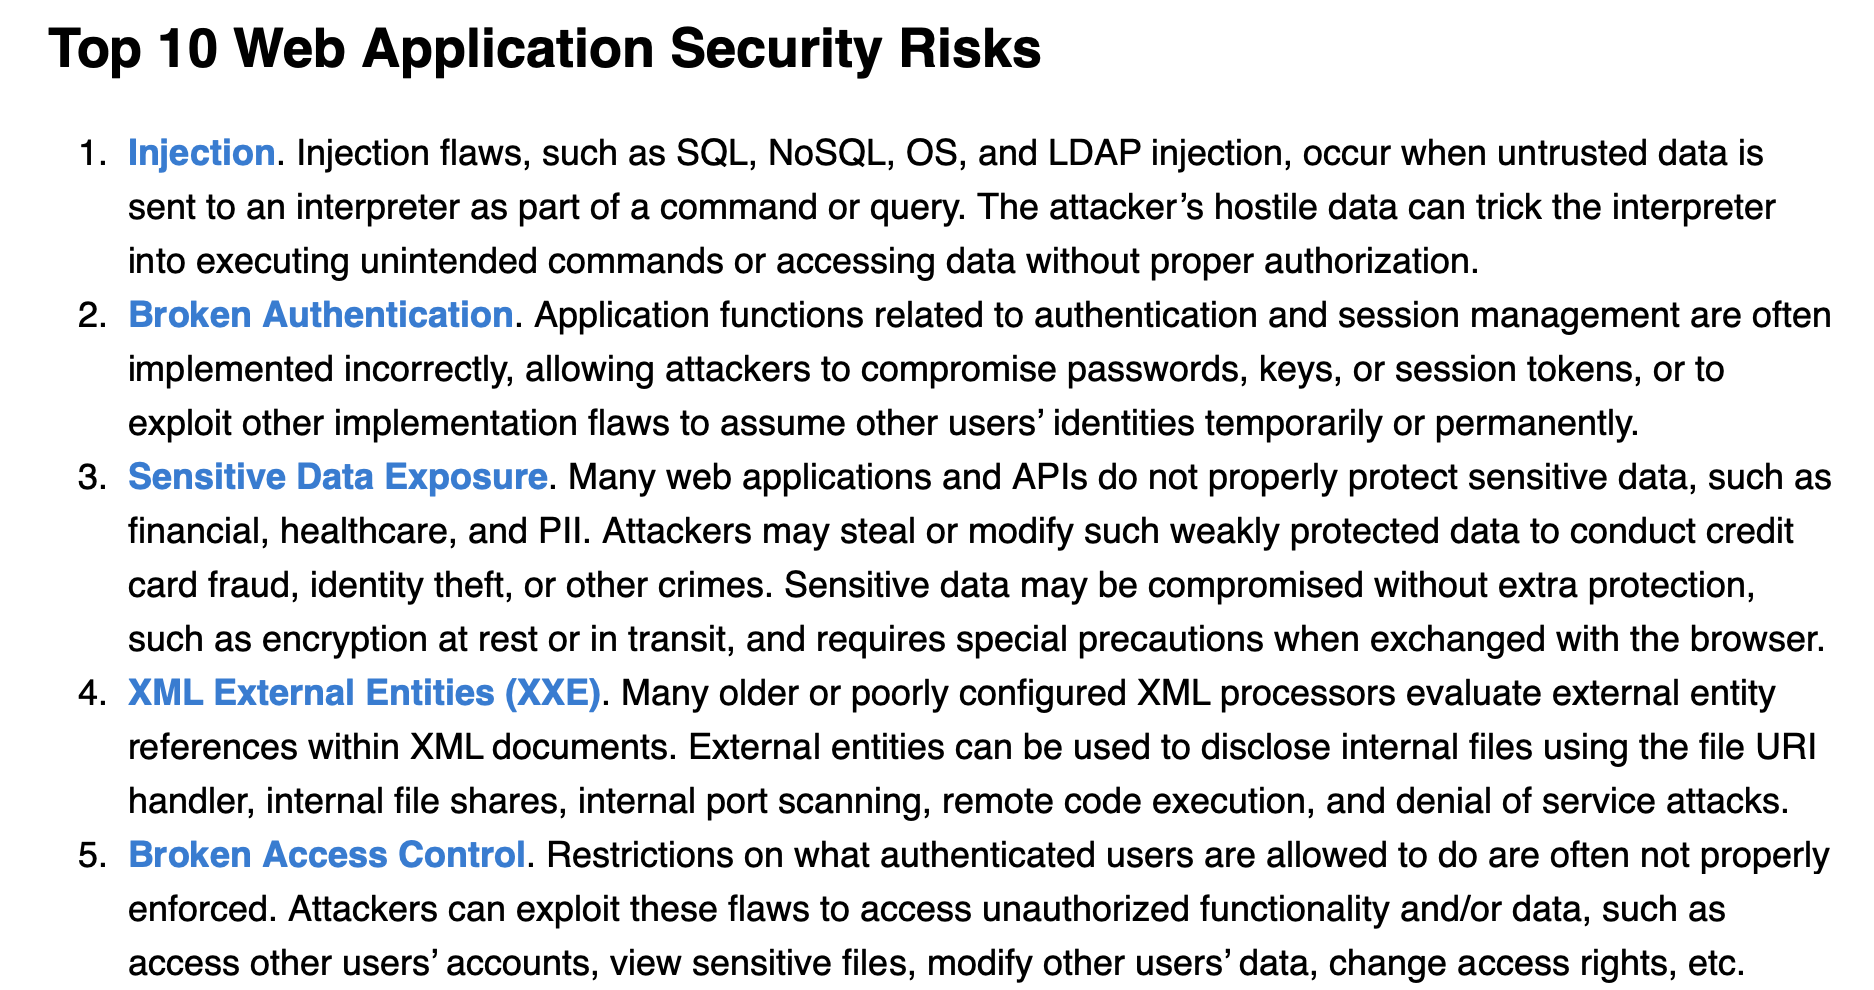
\includegraphics[scale=.35,angle=2]{img/owasp-top10.png}    
    \end{center}
\end{frame}

\begin{frame}
    \frametitle{Fahrplan}

    \begin{itemize}
        \item Get to know your target
        \item Test for stateful attacks
        \item Test for attacks on authentication
        \item Test for cross-site-scripting (XSS)
        \item Test for SQL injection
        \item Test for other injection-based vulnerabilities
        \item Test for attacks on file operations
        \item Test for buffer overflows, format strings and integer bugs
        \item Test for architectural attacks
        \item Test for attacks on the web server 
    \end{itemize}

\end{frame}

\section{0x2: Recon}

{
%\setbeamercolor{background canvas}{bg=yellow}
\usebackgroundtemplate{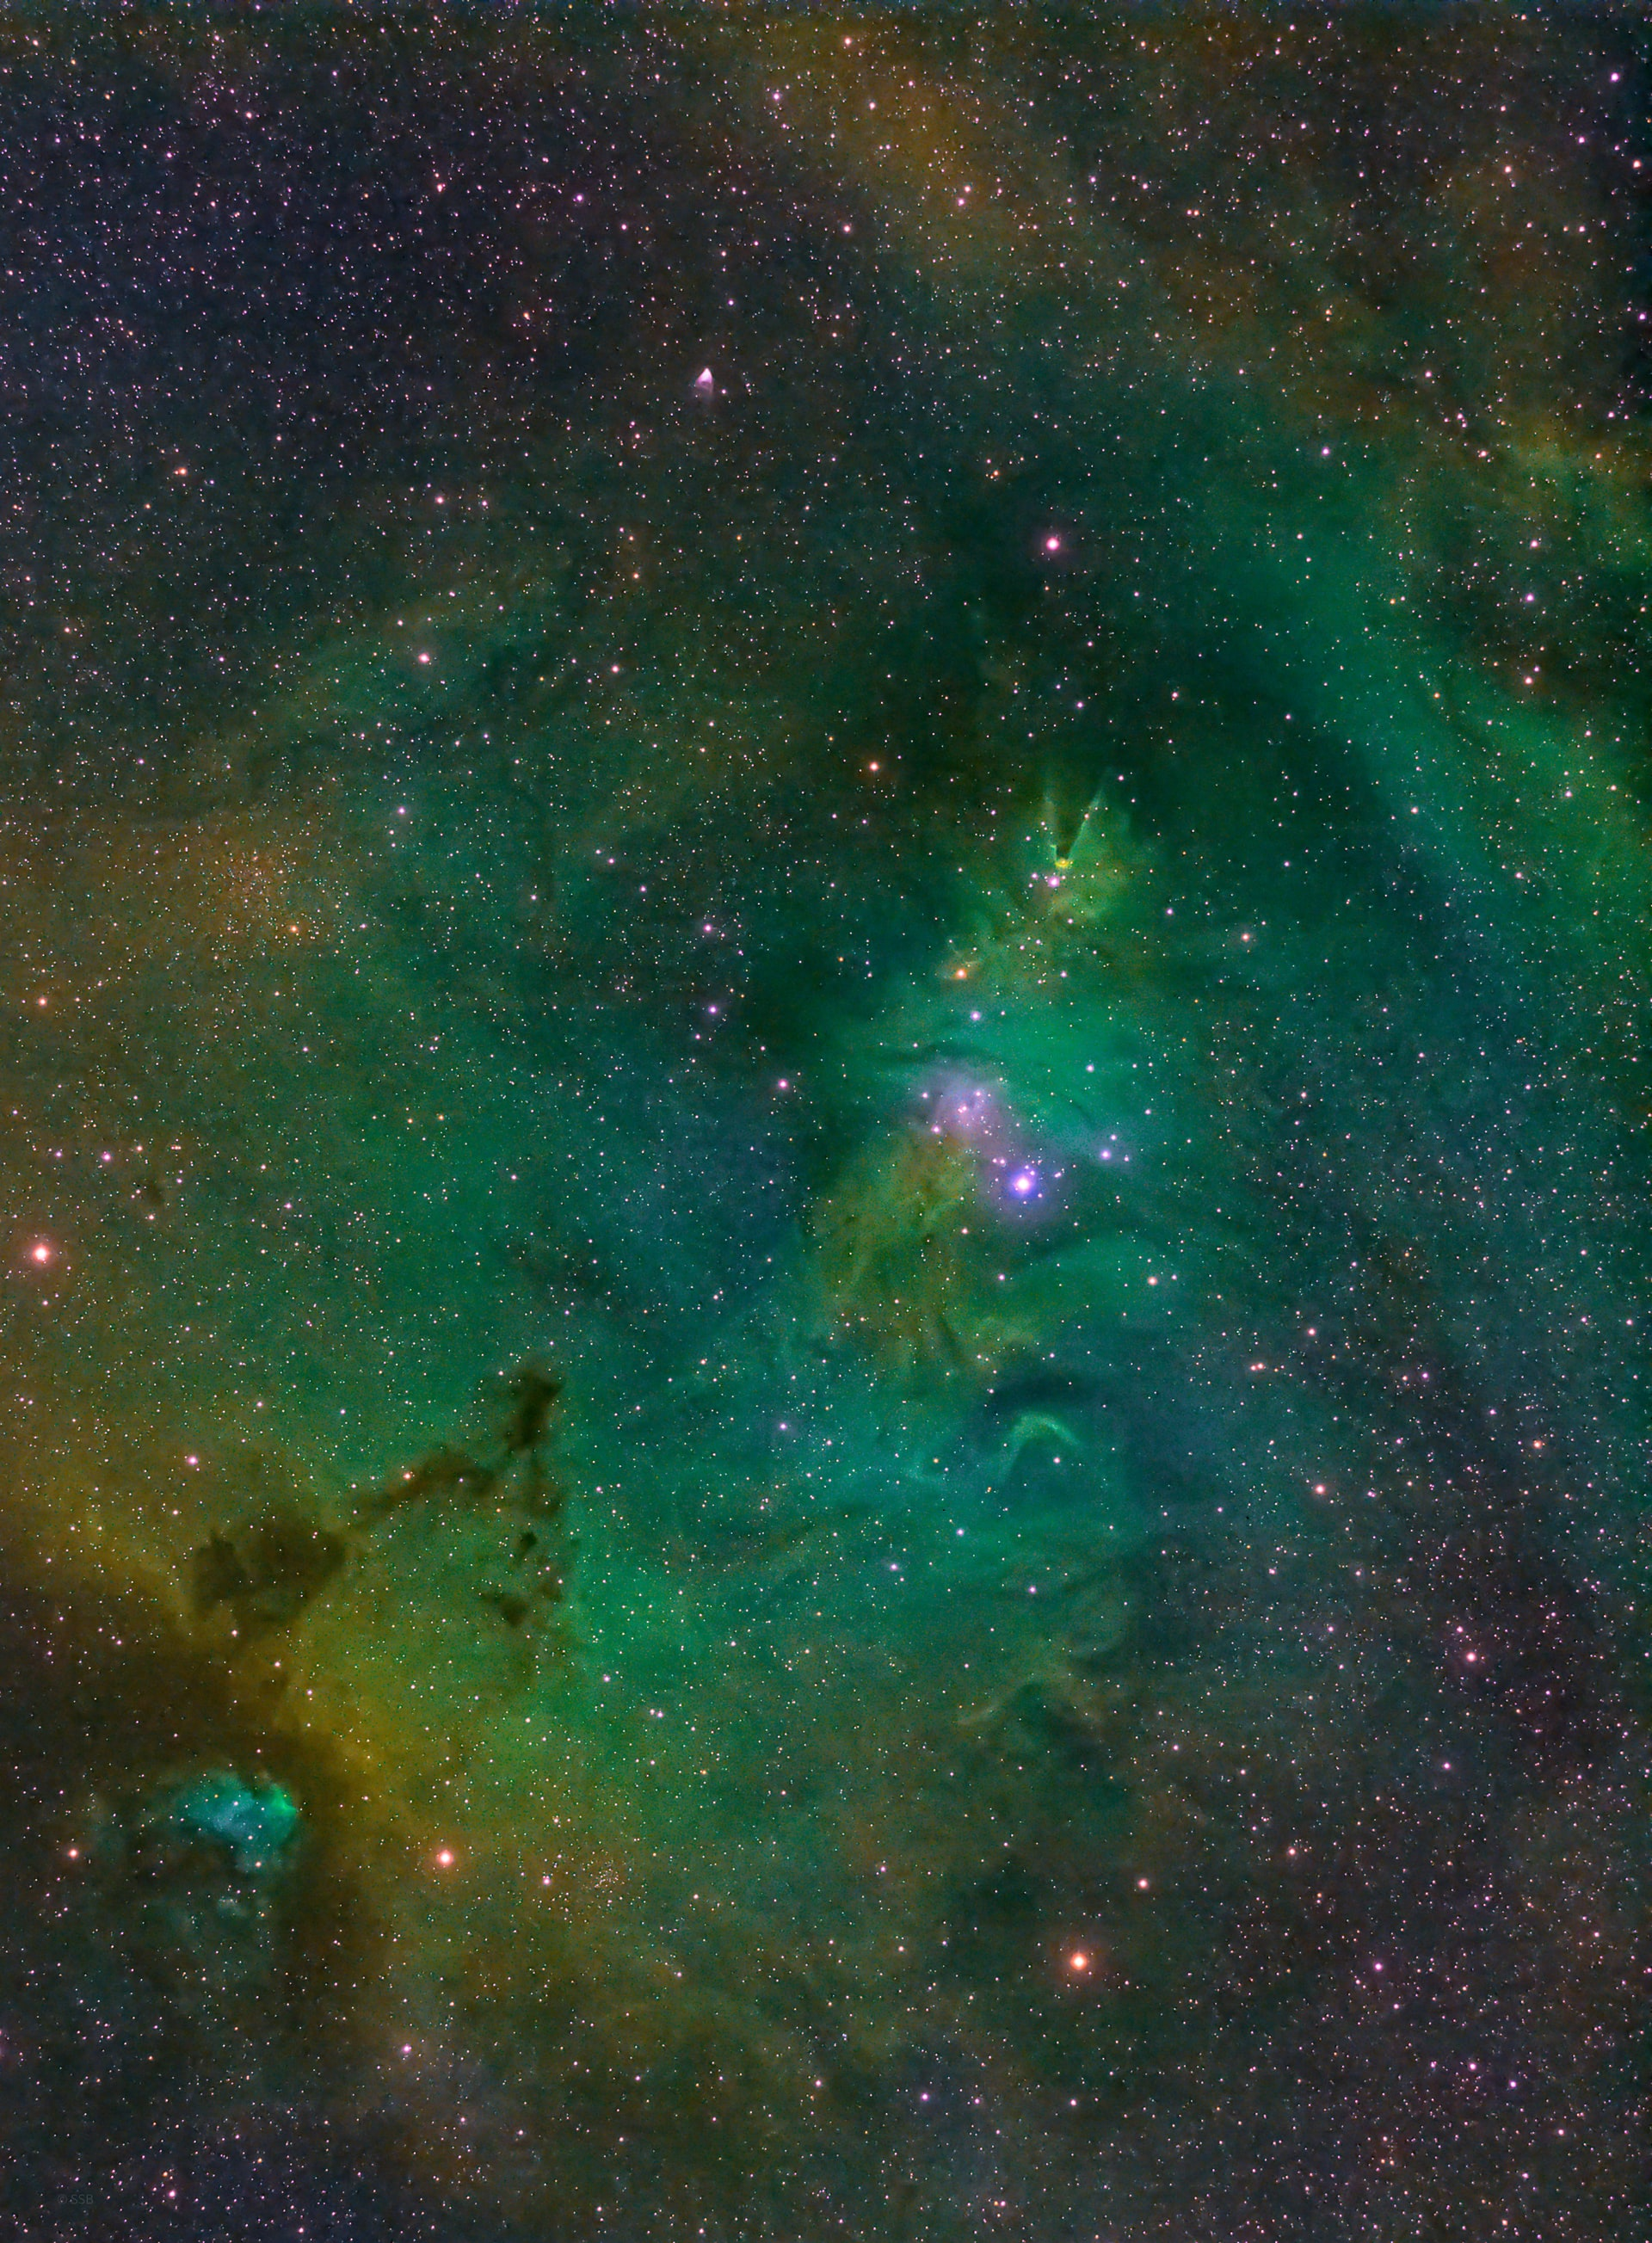
\includegraphics[width=\paperwidth]{./img/aldebaran.jpg}}
\begin{frame}
%\hspace{0.0cm}
\huge{\textcolor{white}{\textbf{0x2: Recon}}}
\end{frame}
}

%\usebackgroundtemplate{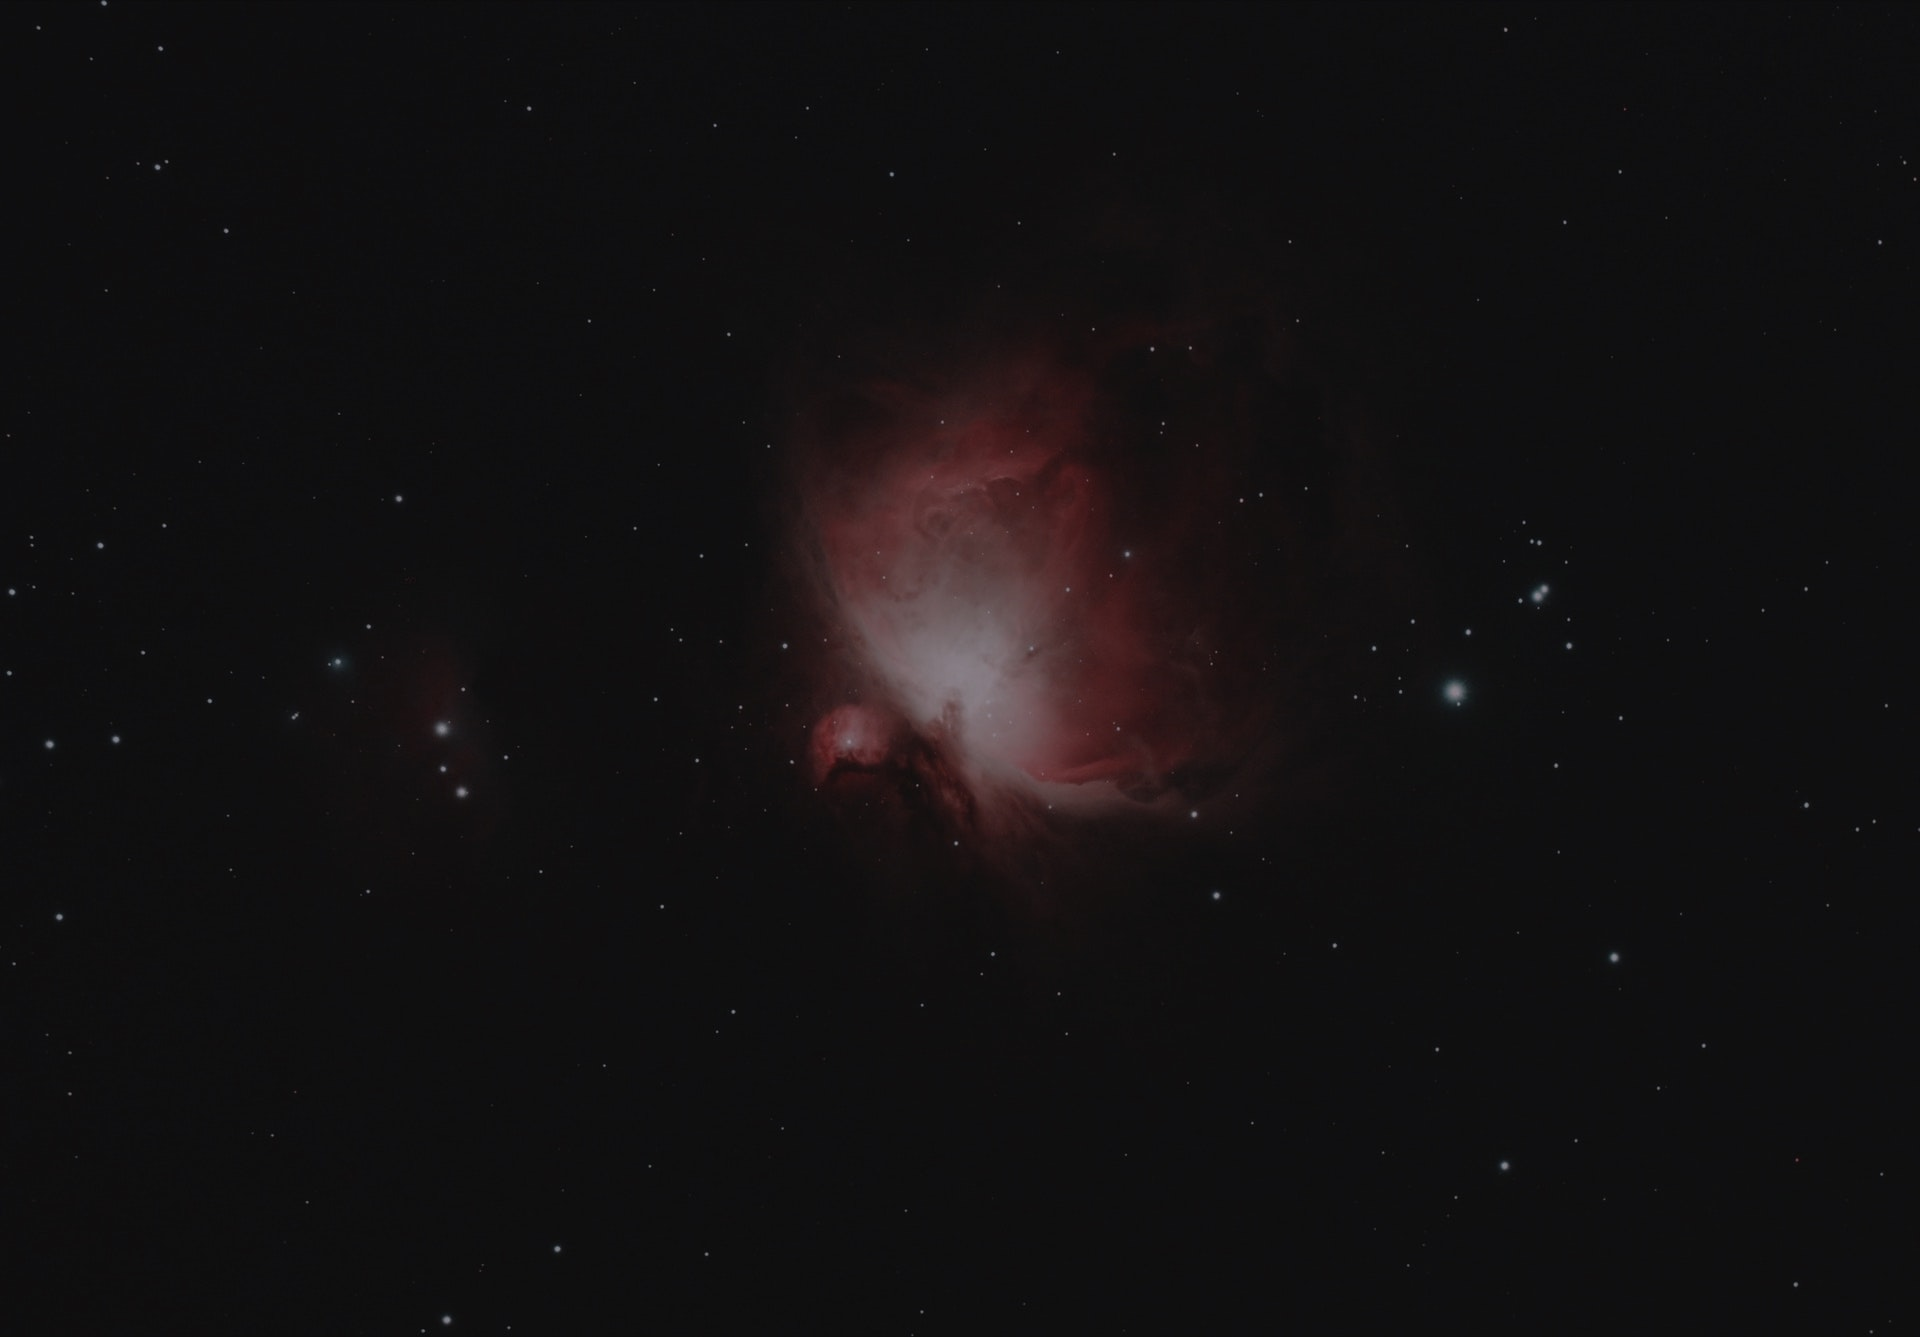
\includegraphics[width=\paperwidth]{./img/orion-nebula-copy.jpg}}

\begin{frame}%{Reconnaissance}
    \textbf{reconnaissance}: \textit{n}. 1. Military observation of a region to locate an enemy or ascertain strategic features. 2. Preliminary surveying or research.
\end{frame}

\begin{frame}
    \frametitle{Why Reconnaissance?}
    \begin{center}
        {\fontsize{70}{80}\selectfont \faQuestionCircle}
        \vfill
        Hint: consider the anatomy of a typical cybersecurity attack.
    \end{center}
\end{frame}

\begin{frame}
    \frametitle{Kill Chain}
    The term \href{https://en.wikipedia.org/wiki/Kill_chain}{kill chain} was originally coined by the military to describe the structure of an attack: finding adversary targets suitable for engagement; fixing their location; tracking and observing; targeting with a suitable weapon or asset to create desired effects; engaging the adversary; assessing the effects;
    \vfill
    In 2011, Hutchins et al~\cite{hutchins2011intelligence} from Lockheed-Martin expanded this concept to an \textbf{intrusion kill chain} for (network) security. They defined intrusion kill chain as reconnaissance, weaponization, delivery, exploitation, installation, command and control (C2), and actions on objectives. 
    \vfill
    Later on, security organizations have adopted this concept under the name "cyber kill chain".
\end{frame}

\begin{frame}
    \frametitle{Intrusion Kill Chain}
    \begin{figure}
        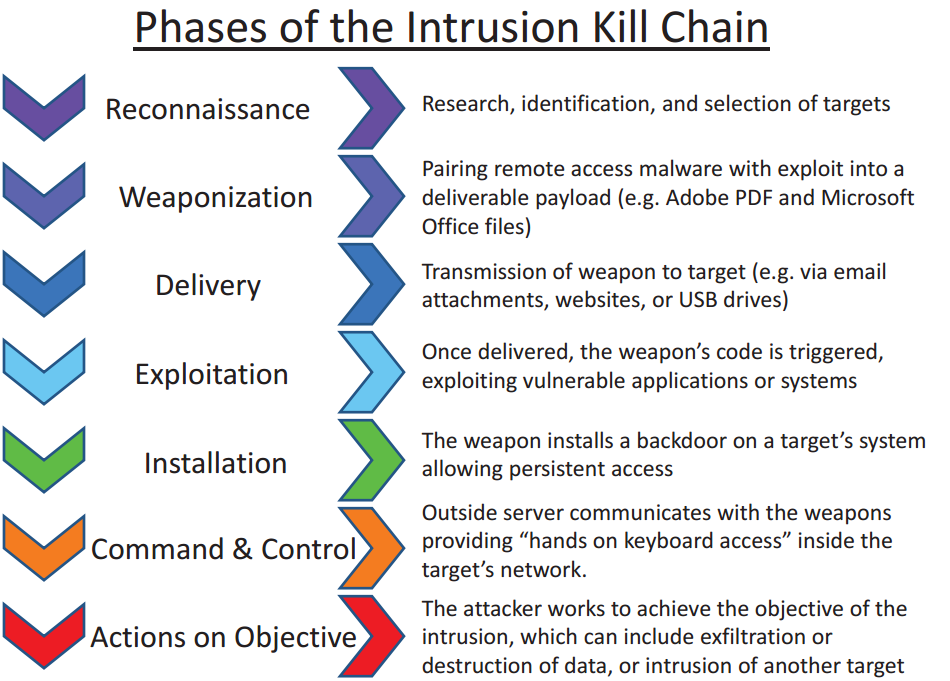
\includegraphics[scale=.35]{img/intrusion-kill-chain.png}
    \end{figure}
    \vfill
    \small{Source: \href{https://commons.wikimedia.org/wiki/File:Intrusion_Kill_Chain_-_v2.png}{Wikimedia Commons}.}
\end{frame}

\begin{frame}
    \frametitle{Mimicking the Attacker}
    Every attack starts by collecting information about the target, e.g., a web application ($\rightarrow$ cyber kill chain).
    \vfill
    Likewise, to test a web application for security vulnerabilities, you must first get to know it. You must understand what functions it uses and what parameters these functions have. You have to test every parameter whether it can be exploited (e.g., using illegitimate values). You need to check whether the web application code contains known vulnerabilities.
    \vfill
    \textbf{Systematic collection and documentation} allows you to understand what a real attacker would learn and where she could break your application's security.
\end{frame}

\begin{frame}
    \frametitle{Collecting Rudimentary Information}
    Document any \textbf{easy-to-spot hints} to security vulnerabilities:
    \begin{itemize}
        \item Suspicious comments in the HTML code (\texttt{<!-- default password:...})
        \item Sensitive information embedded in the HTML code
        \item Error messages from the web application
        \item Error messages from the webserver and http responses
    \end{itemize}
\end{frame}


\begin{frame}
    \frametitle{Learning the Web Application Structure}
    Catalogue \textbf{all pages, resources and parameters} that belong to or are used by the web application:
    \begin{itemize}
        \item using a general-purpose tool like \href{https://www.gnu.org/software/wget/}{\texttt{wget}}
        \item using a special-purpose tool like the \href{https://www.zaproxy.org/}{OWASP Zed Attack Proxy (ZAP)} crawler
        \item by manually visiting all web pages of the application (works well for small web applications)
    \end{itemize}
    \vfill
    While \texttt{GET} parameters are displayed in the URL, you'll need a web proxy like OWASP ZAP to access \texttt{POST} parameters and cookies.
    \vfill
    If your web application has different roles (guest, admin, \ldots), you'll have to test it for all these roles (i.e., first as a guest, then logged in as admin, etc.)
\end{frame}

\begin{frame}
    \frametitle{Investigating Individual Web Pages}
    Visit all pages and \textbf{inspect their source code}. Look for things like:
    \begin{itemize}
        \item \textbf{Leaky HTML comments} (comments containing e.g., code fragements, configuration parameters, server names, SQL table descriptions, etc.)
        \item \textbf{Hidden input fields} (\texttt{<input type='hidden' ...>})
        \item \textbf{SQL queries} printed in the page source due to programming or configuration errors (reveal the structure of the database and the queries used)
        \item \textbf{IP addresses of internal servers}
        \item \textbf{Web or email addresses}, e.g., email addresses of the developers (might reveal who wrote the application. Maybe it's just an optical tweak of a well-known application?)
    \end{itemize} 
    

\end{frame}

\begin{frame}
    \frametitle{Investigating Parameters}
    Investigate \textbf{all parameters} passed to the application:
    \begin{itemize}
        \item What happens when you change their values or use invalid values, e.g., a string instead of an integer?
        \item Do invalid parameters return error message that leak information about the application like database table names?
    \end{itemize}
\end{frame}

\begin{frame}
    \frametitle{Collecting More Information}
   \begin{itemize}
       \item Are there unlinked resources likes directories or files?
       \item E.g., if there are links to files financial-report18.pdf and financial-report19.pdf, is there an unpublished file financial-report20.pdf?
       \item Are there any hints to the structure of file names or subdirectories?
       \item E.g., if the web application contains user profiles, is it possible to access an arbitrary profile using \texttt{user-[number].html} or \texttt{user.php?id=[number]}?
       \item Are there unlinked subdirectories like \texttt{test/} or \texttt{admin/}?
       \item Does the webserver contain unused libraries or example application code that contains hints to known vulnerabilities or the internals of the web application? 
       \item What else is running on the server? SSH?
   \end{itemize}
\end{frame}

\begin{frame}
    \frametitle{Collecting Client-Side Information}

\end{frame}

\begin{frame}
    \frametitle{Collecting Information about Static Pages}
\end{frame}

\begin{frame}
    \frametitle{Collecting JavaScript-related Information}
\end{frame}

\begin{frame}
    \frametitle{Sample frame title}
    
    In this slide, some important text will be
    \alert{highlighted} because it's important.
    Please, don't abuse it.
    
    \begin{block}{Remark}
    Sample text
    \end{block}
    
    \begin{alertblock}{Important theorem}
    Sample text in red box
    \end{alertblock}
    
    \begin{examples}
    Sample text in green box. The title of the block is ``Examples".
    \end{examples}

\end{frame}

\begin{frame}
    \frametitle{Tools}
    \begin{itemize}
        \item ZAProxy
        \item ...
    \end{itemize}
\end{frame}


\begin{frame}
    \frametitle{Example}

    \begin{itemize}
        \item<1-> one
        \item<2-> two
        \item<3-> theorem
    \end{itemize}

\end{frame}

\begin{frame}
    \frametitle{Example 1}
    One \pause
    Two \pause
    Three
\end{frame}

\section{0x3: Stateful Attacks}
{
\usebackgroundtemplate{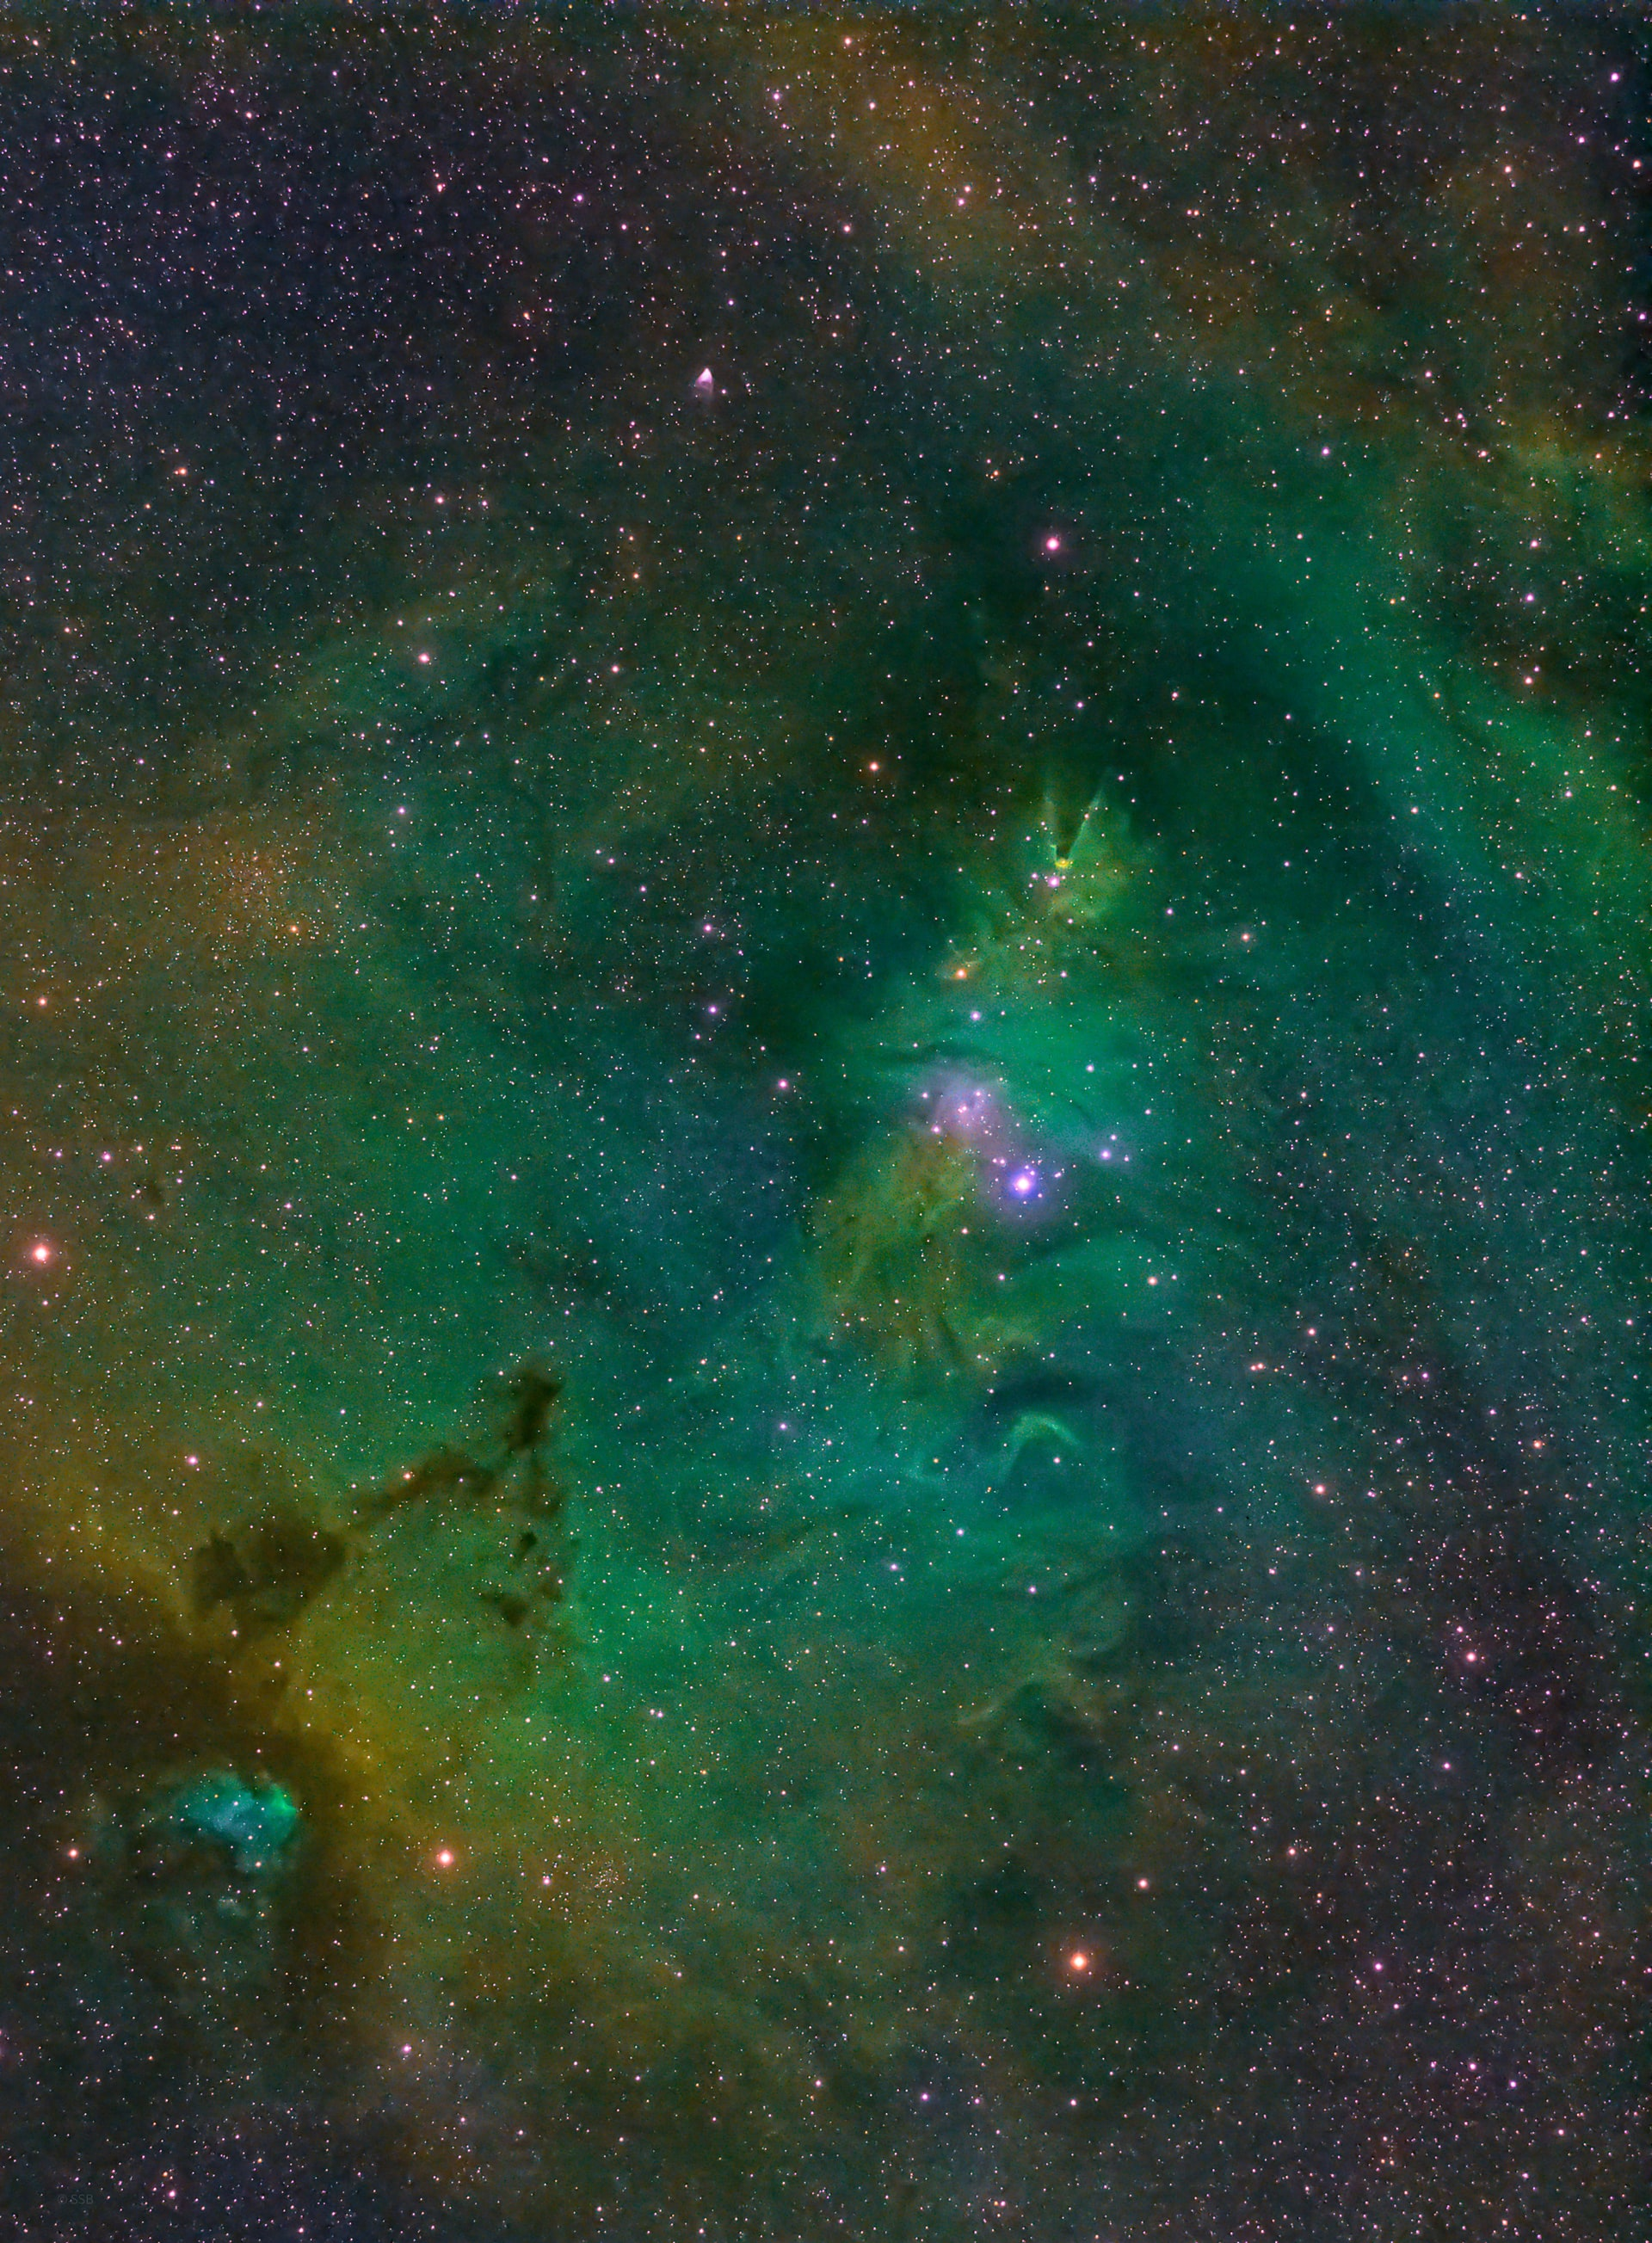
\includegraphics[width=\paperwidth]{./img/aldebaran.jpg}}
\begin{frame}
\huge{\textcolor{white}{\textbf{0x3: Stateful Attacks}}}
\end{frame}
}

\section{0x4: Attacks on Authentication}
{
\usebackgroundtemplate{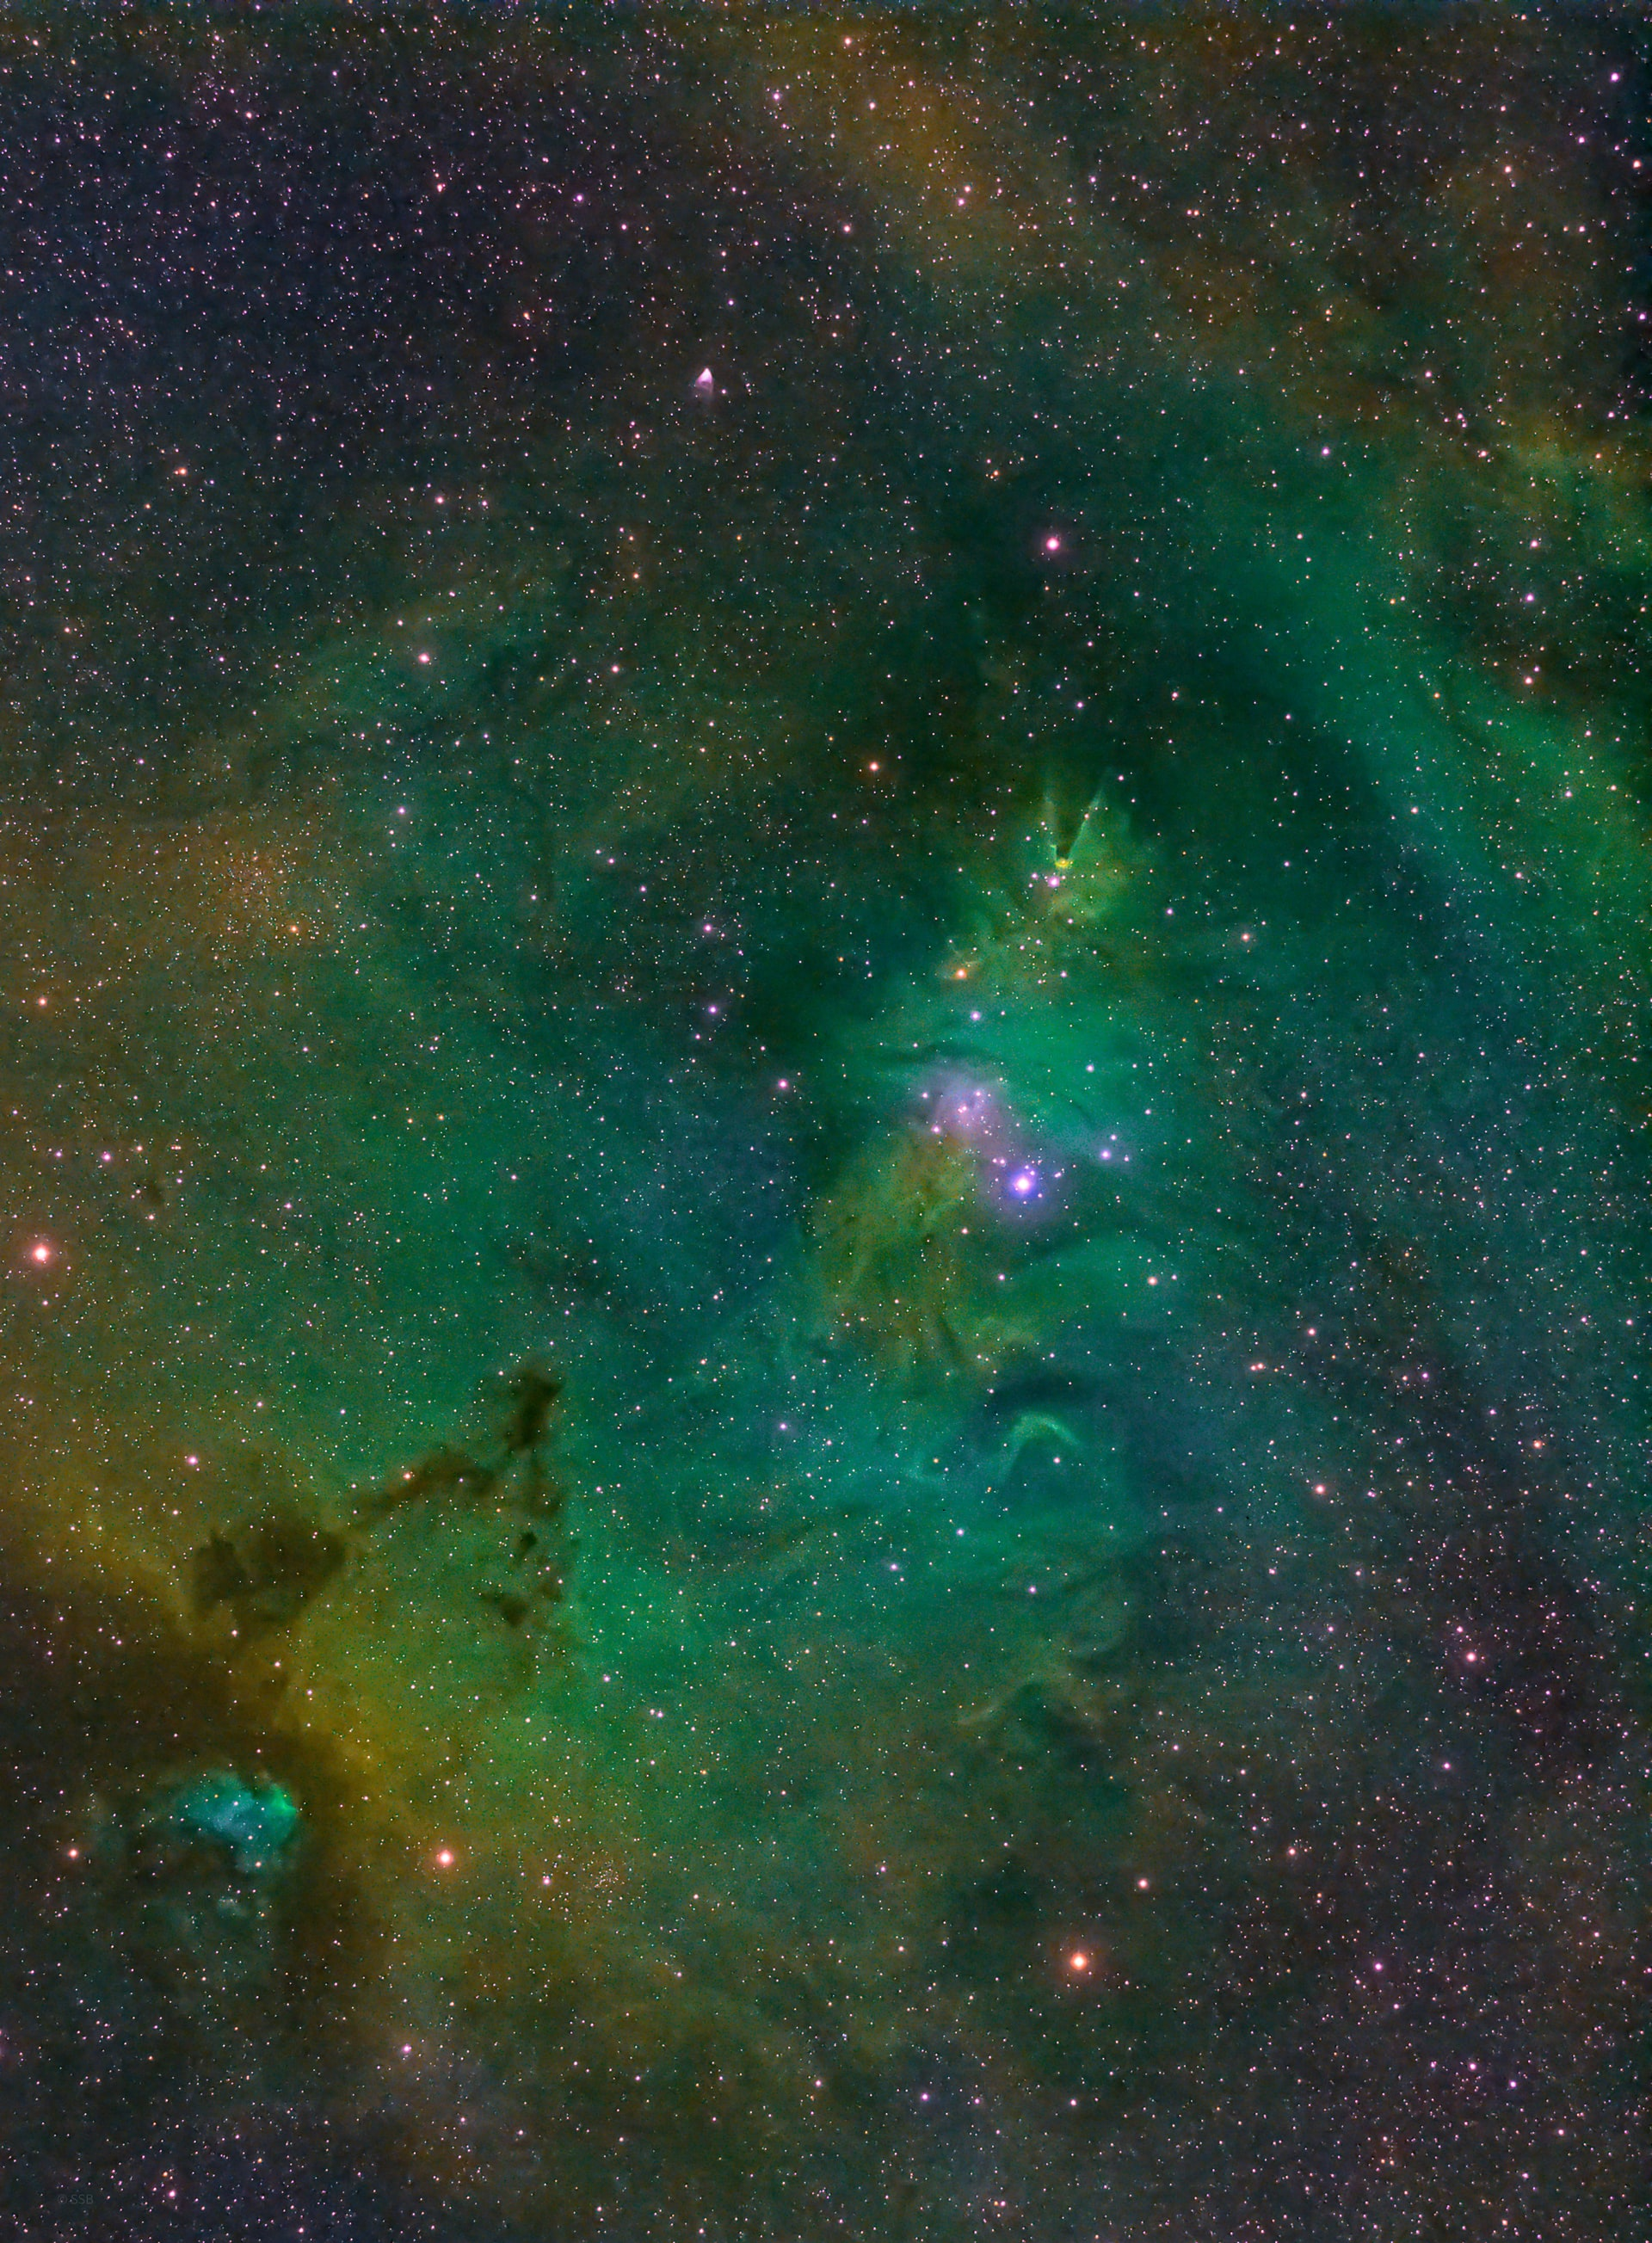
\includegraphics[width=\paperwidth]{./img/aldebaran.jpg}}
\begin{frame}
\huge{\textcolor{white}{\textbf{0x4: Attacks on Authentication}}}
\end{frame}
}

\section{0x5: Cross-Site-Scripting (XSS)}
{
\usebackgroundtemplate{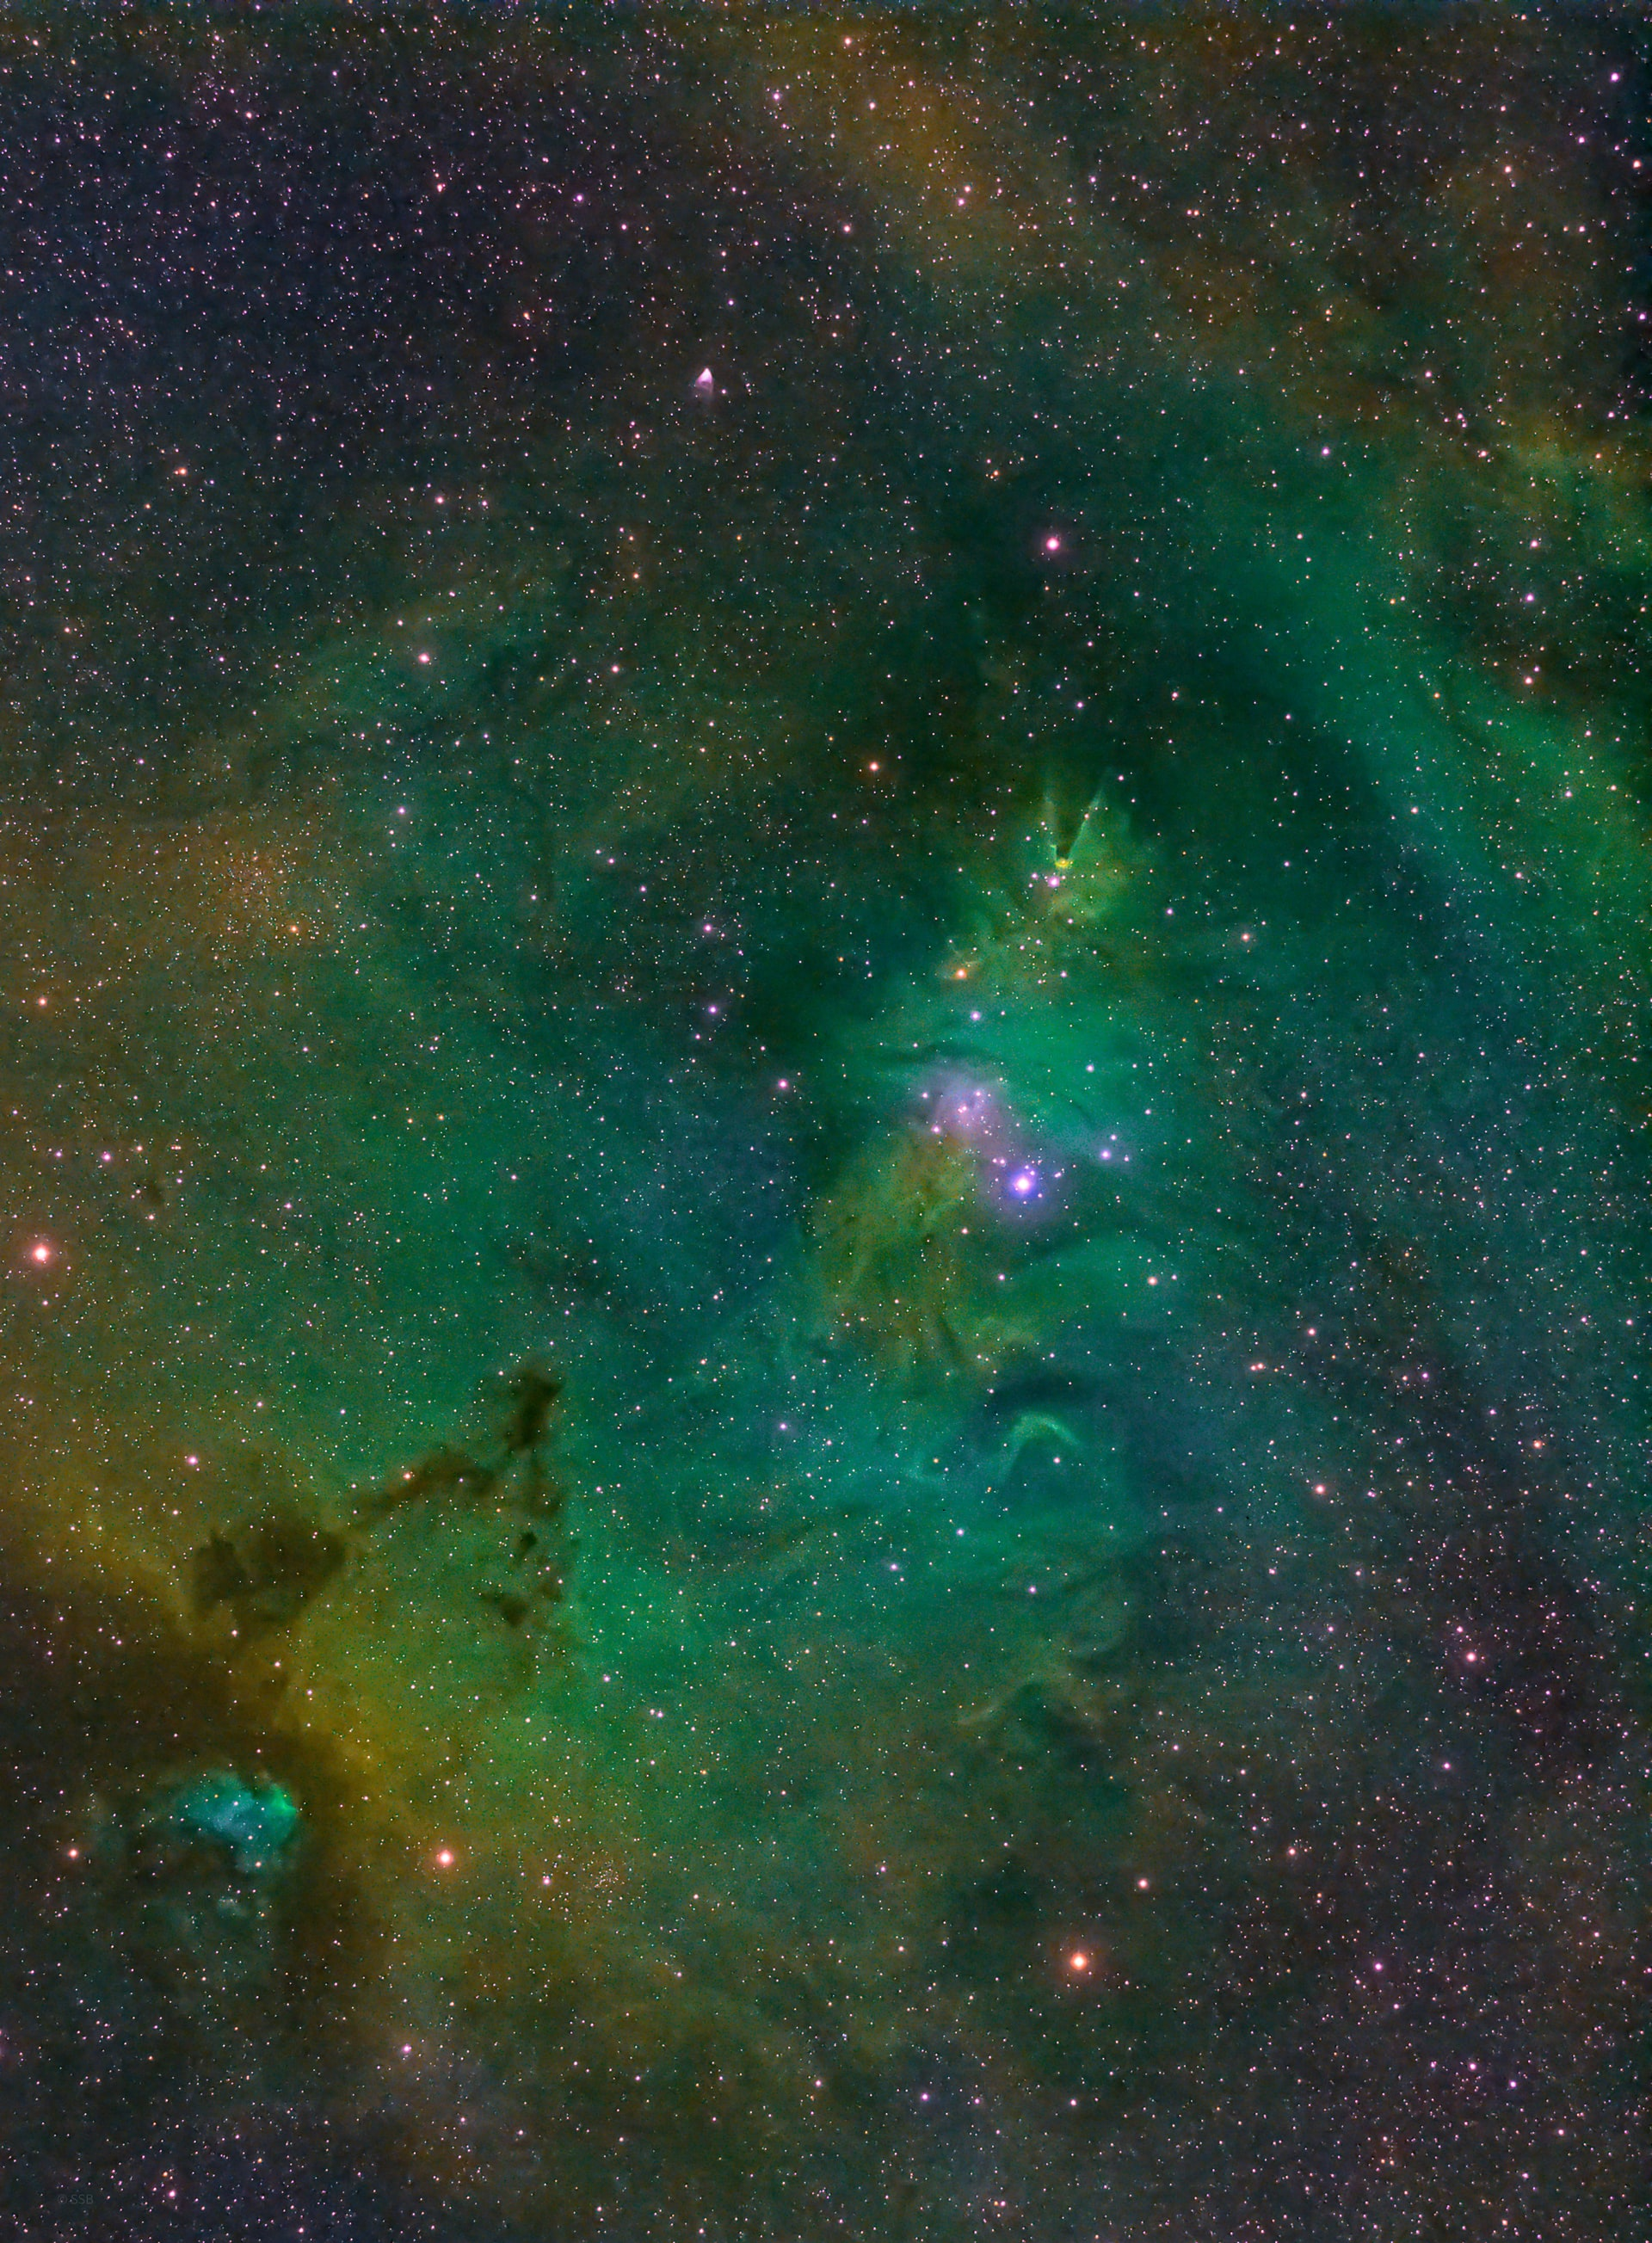
\includegraphics[width=\paperwidth]{./img/aldebaran.jpg}}
\begin{frame}
\huge{\textcolor{white}{\textbf{0x5: Cross-Site-Scripting (XSS)}}}
\end{frame}
}

\section{0x6: SQL Injection}
{
\usebackgroundtemplate{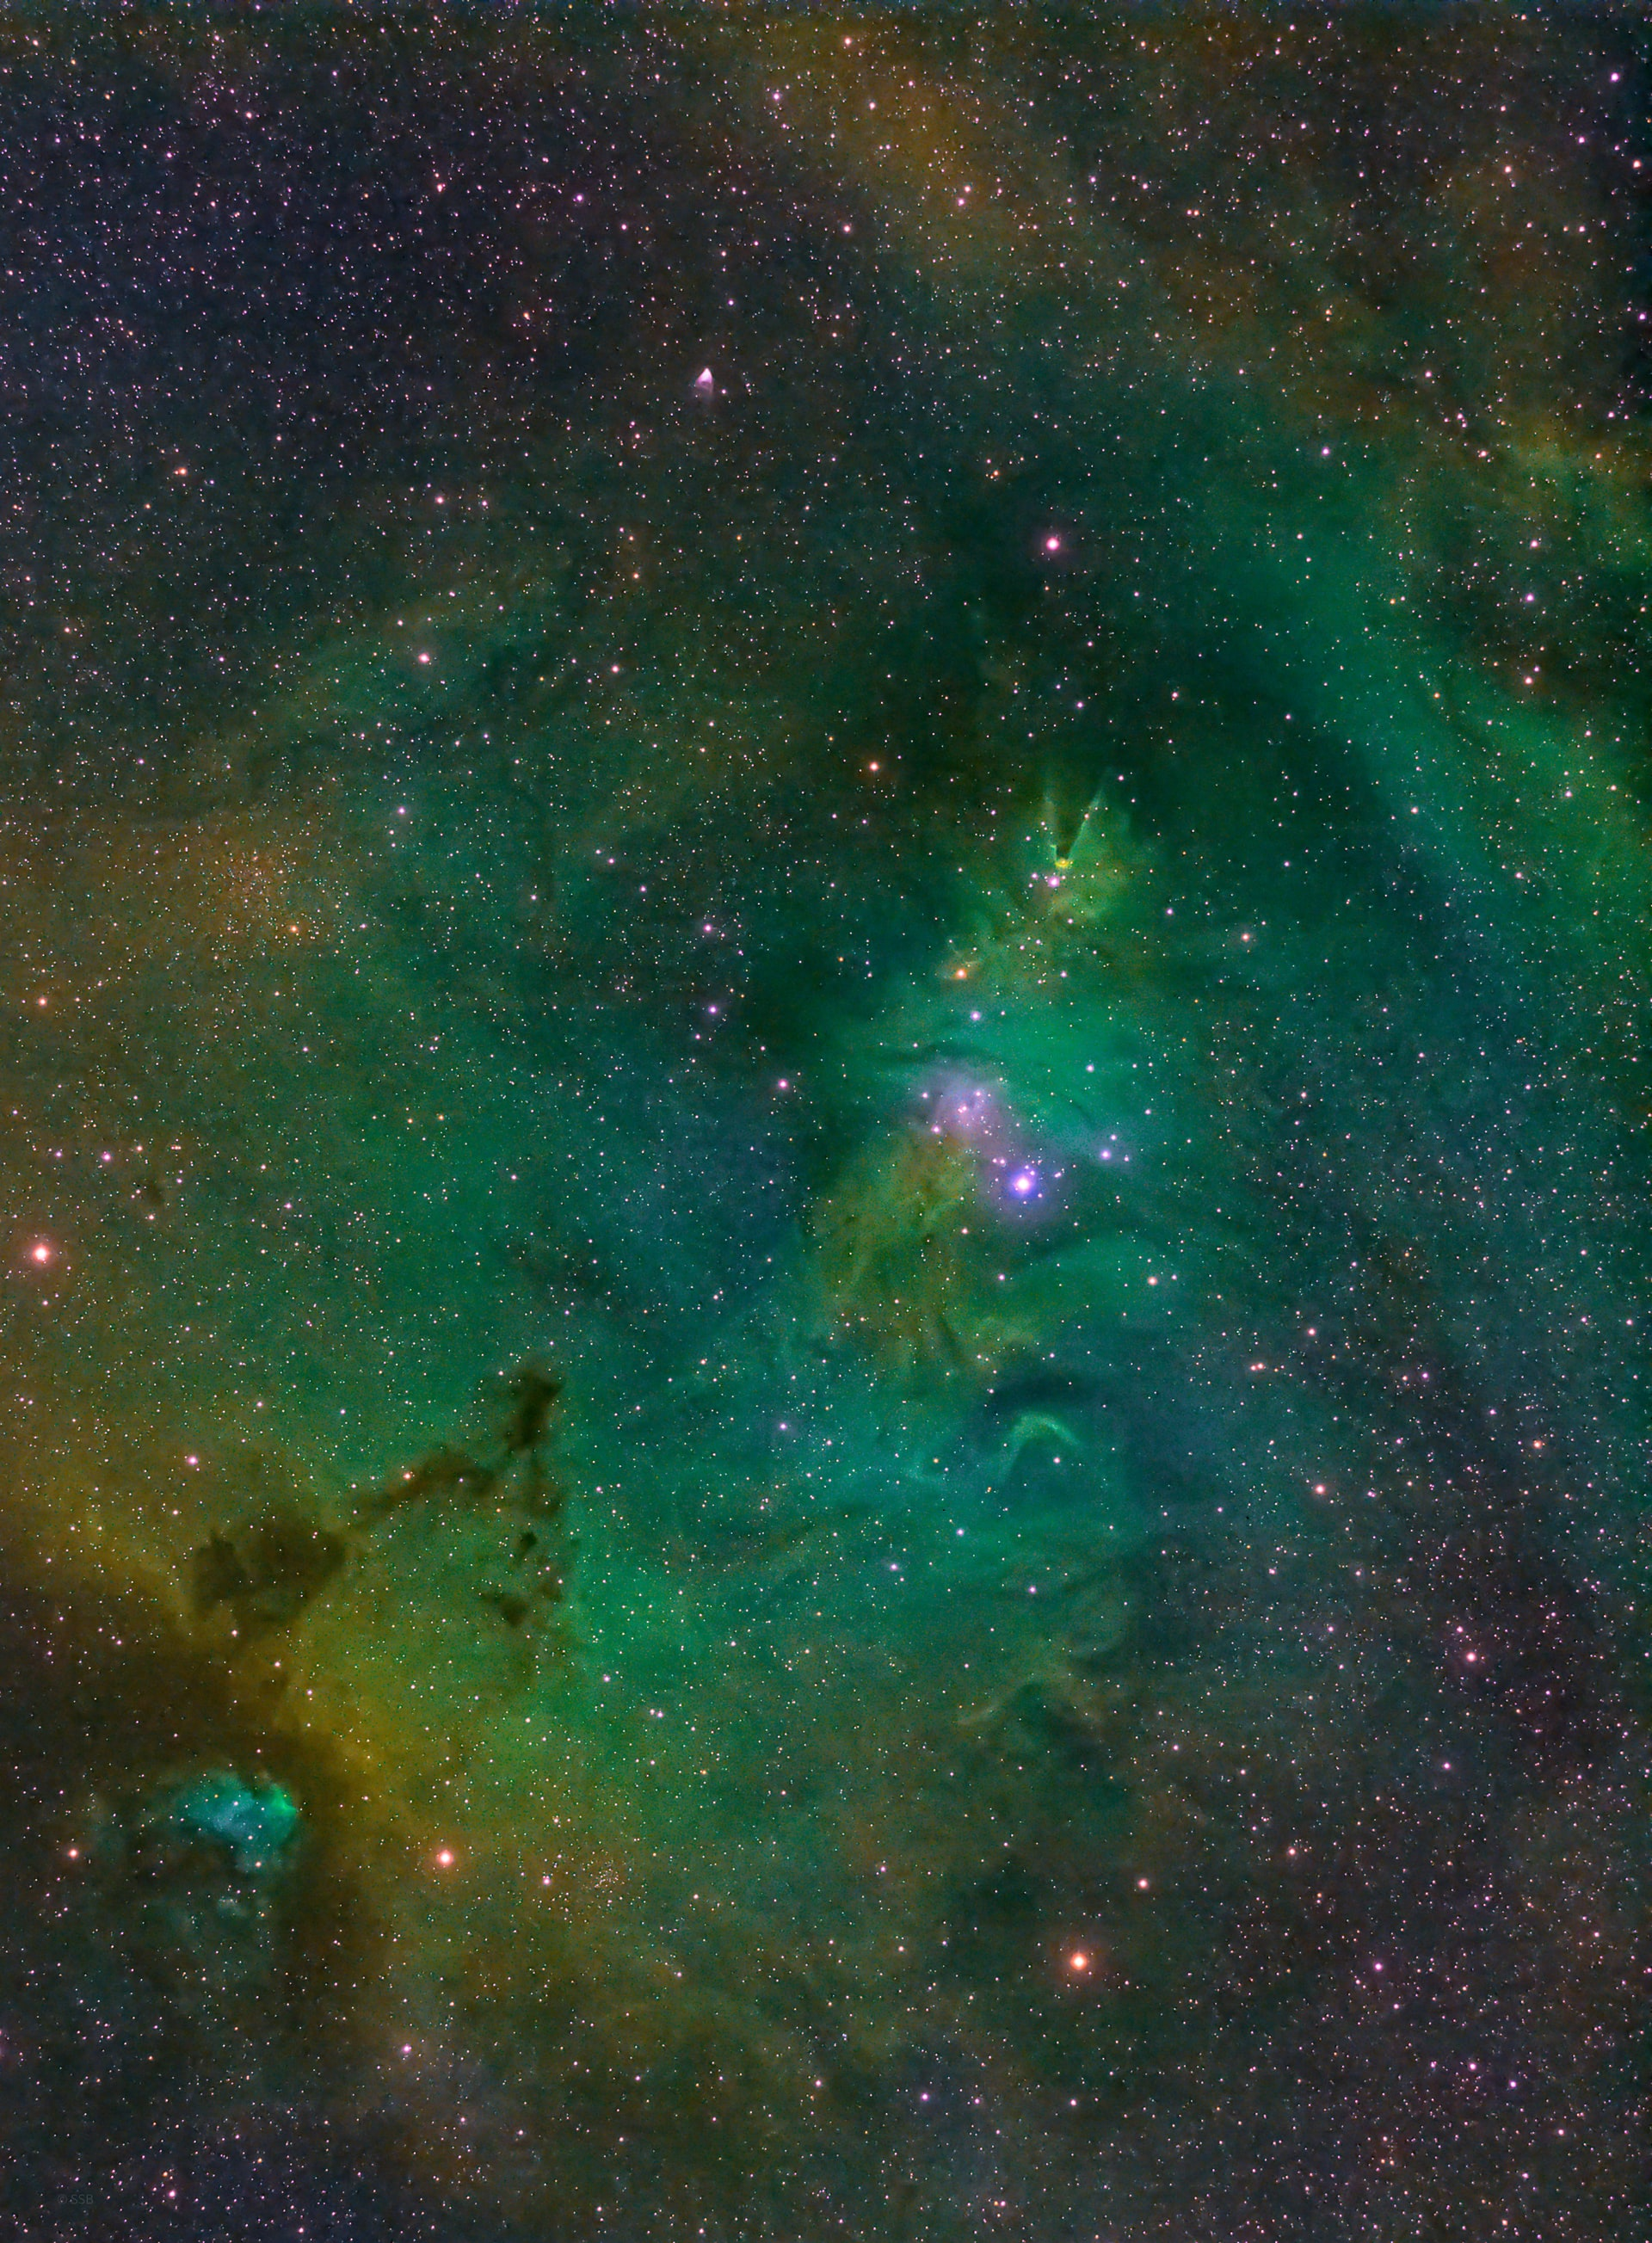
\includegraphics[width=\paperwidth]{./img/aldebaran.jpg}}
\begin{frame}
\huge{\textcolor{white}{\textbf{0x6: SQL Injection}}}
\end{frame}
}

\section{0x7: Other Injection-Based Vulnerabilities}
{
\usebackgroundtemplate{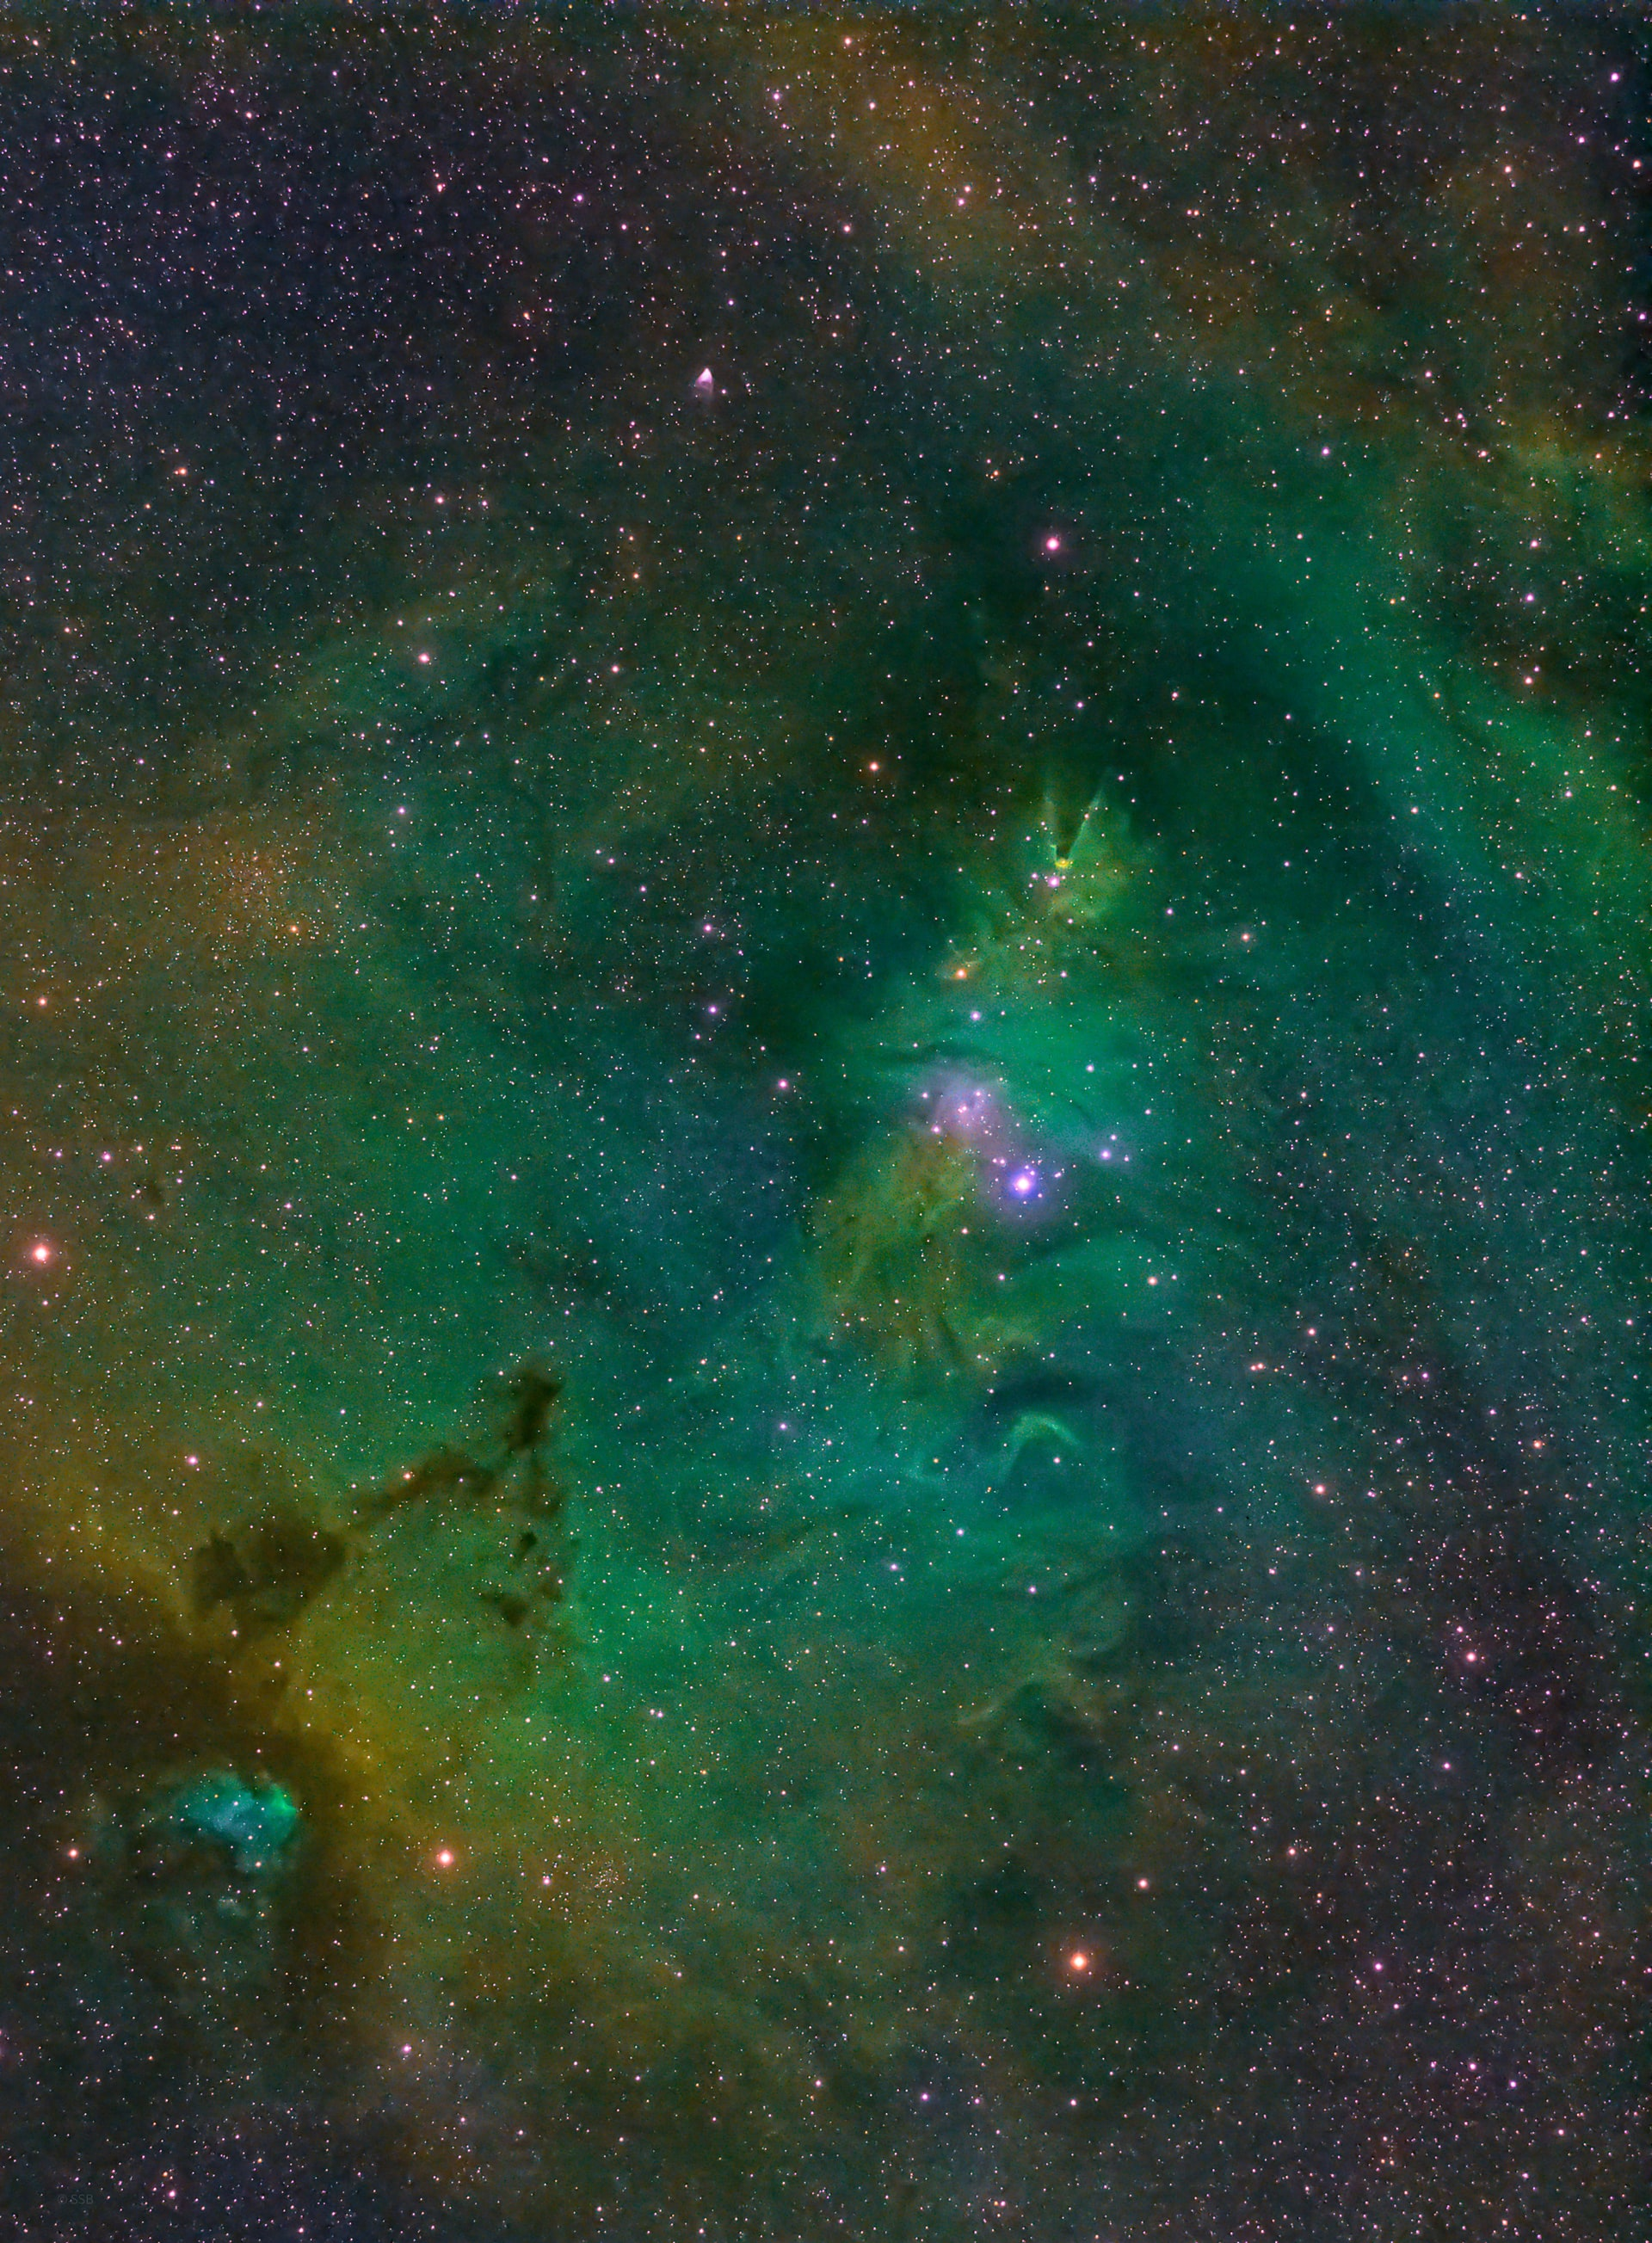
\includegraphics[width=\paperwidth]{./img/aldebaran.jpg}}
\begin{frame}
\huge{\textcolor{white}{\textbf{0x7: Other Injection-Based Vulnerabilities}}}
\end{frame}
}

\section{0x8: Attacks on File Operations}
{
\usebackgroundtemplate{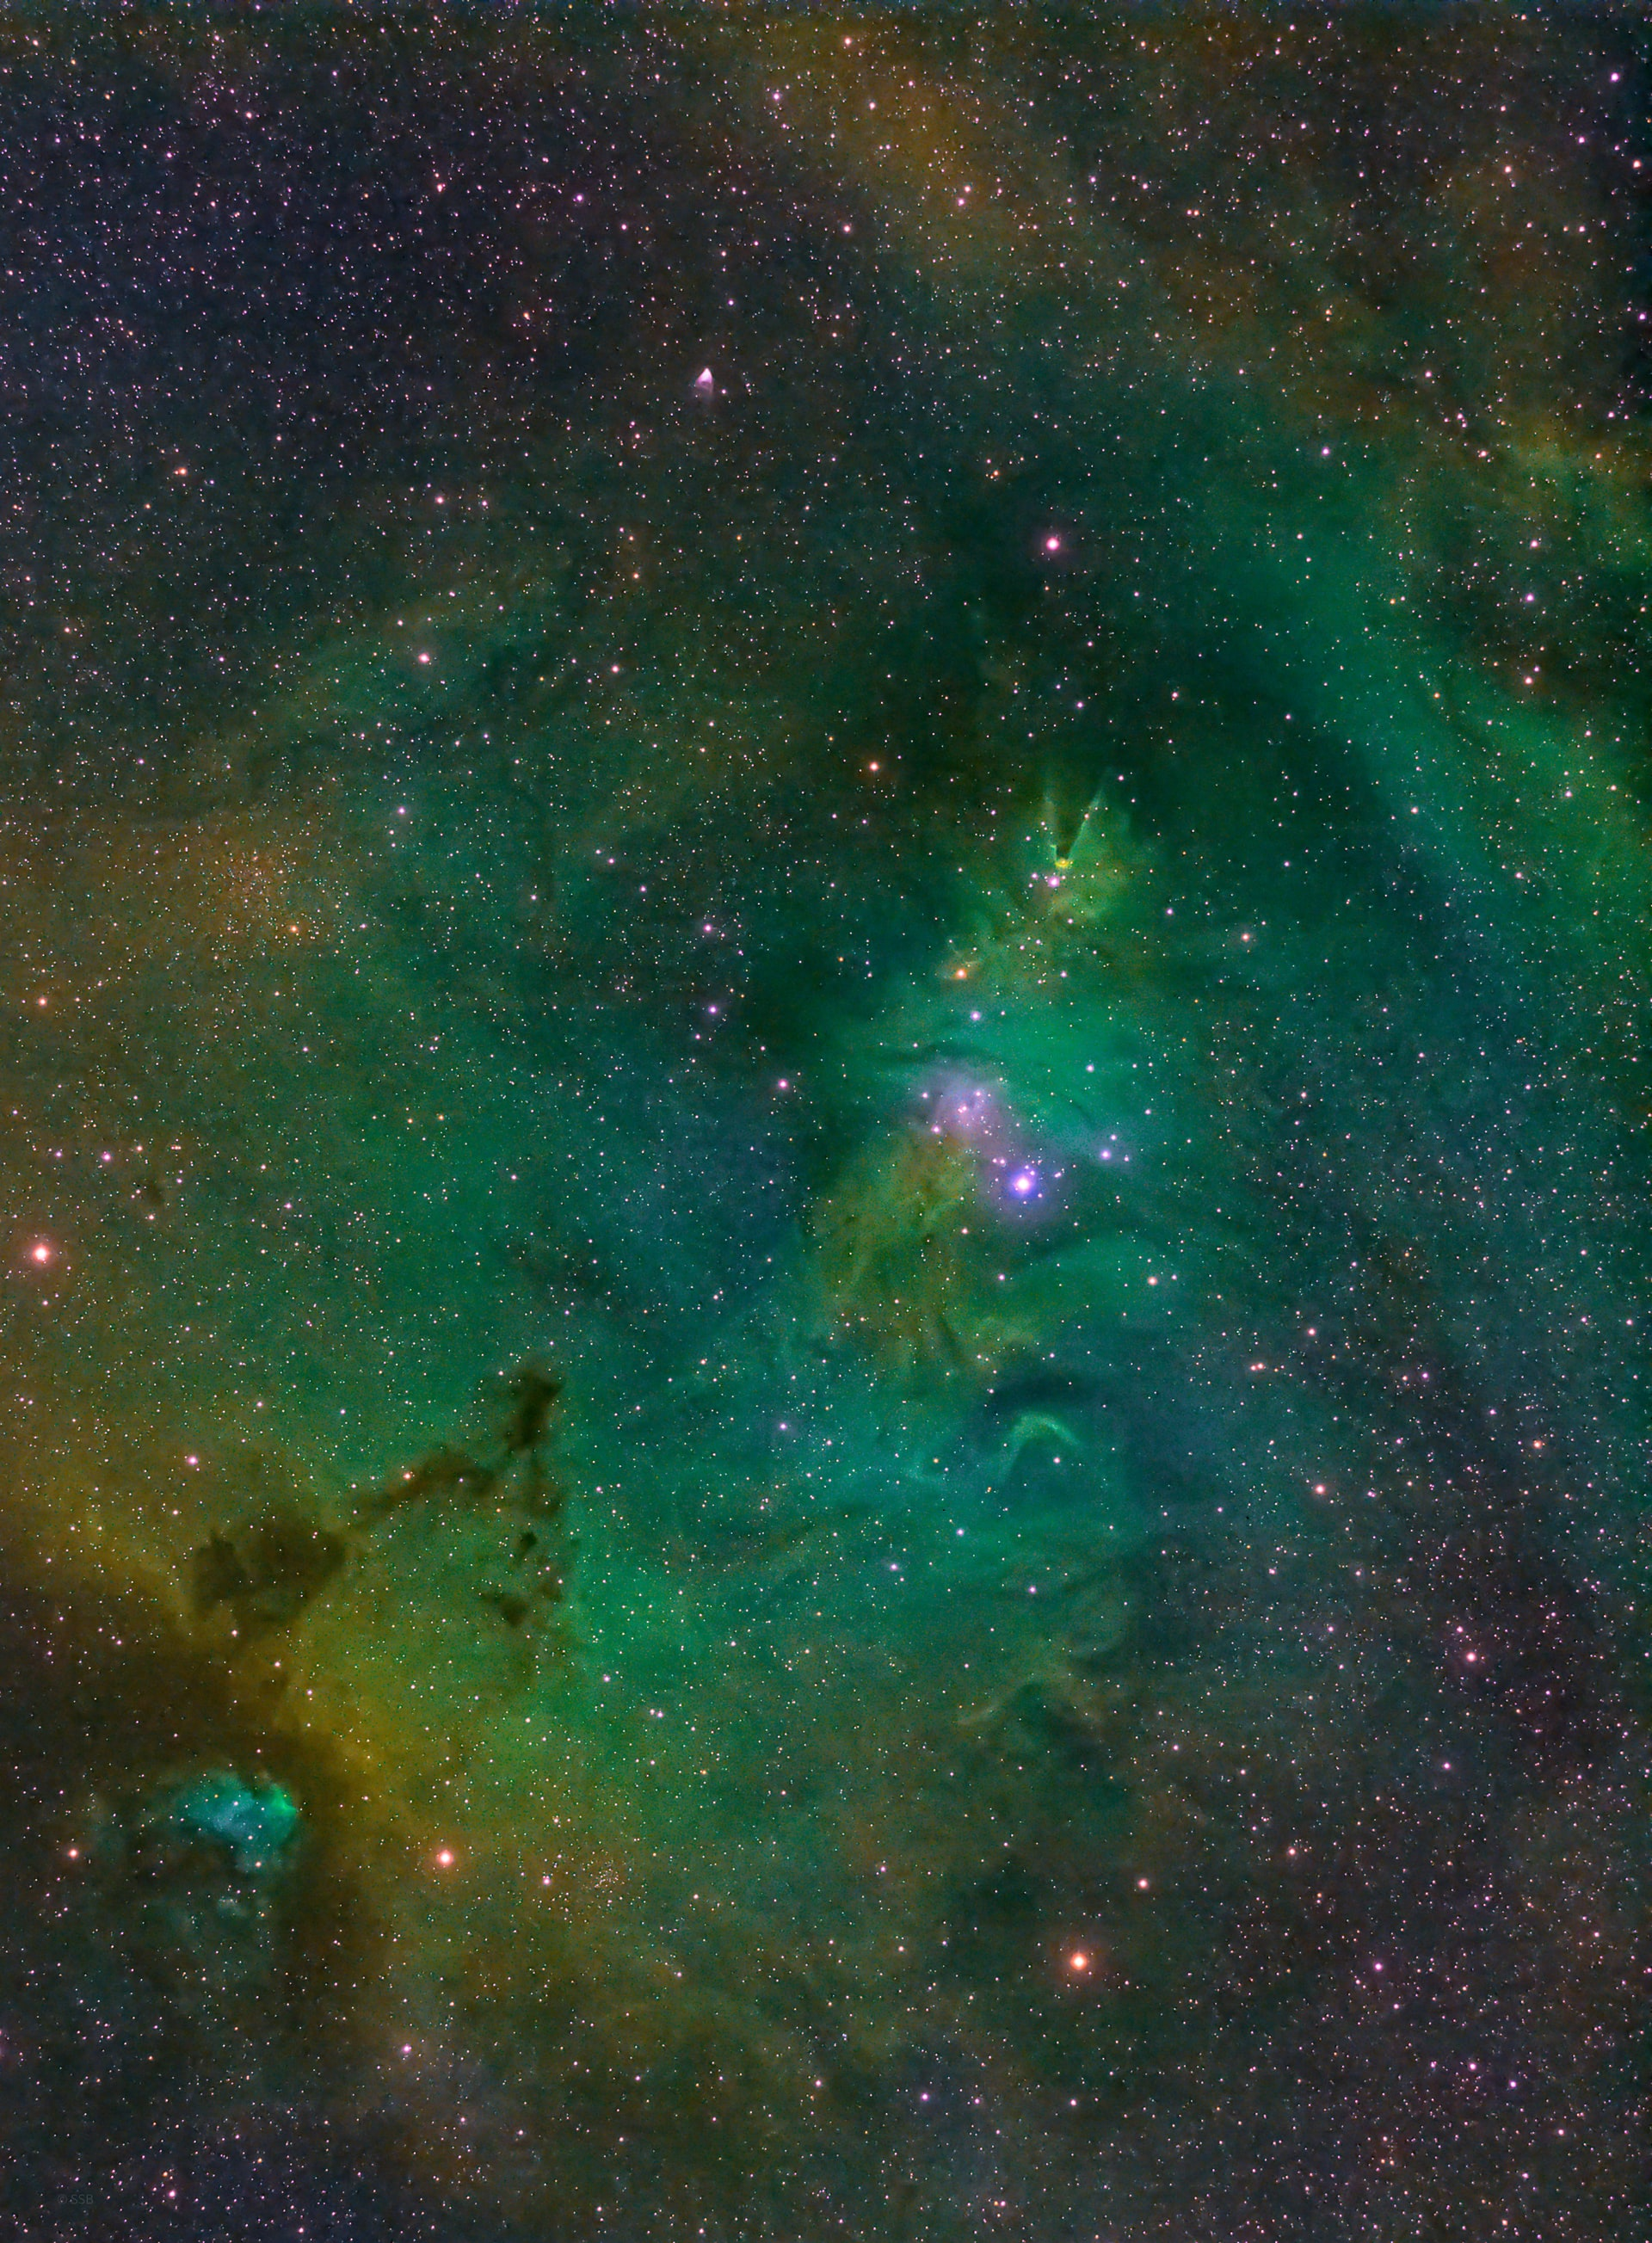
\includegraphics[width=\paperwidth]{./img/aldebaran.jpg}}
\begin{frame}
\huge{\textcolor{white}{\textbf{0x8: Attacks on File Operations}}}
\end{frame}
}

\section{0x9: Buffer Overflows, Format Strings and Integer Bugs}
{
\usebackgroundtemplate{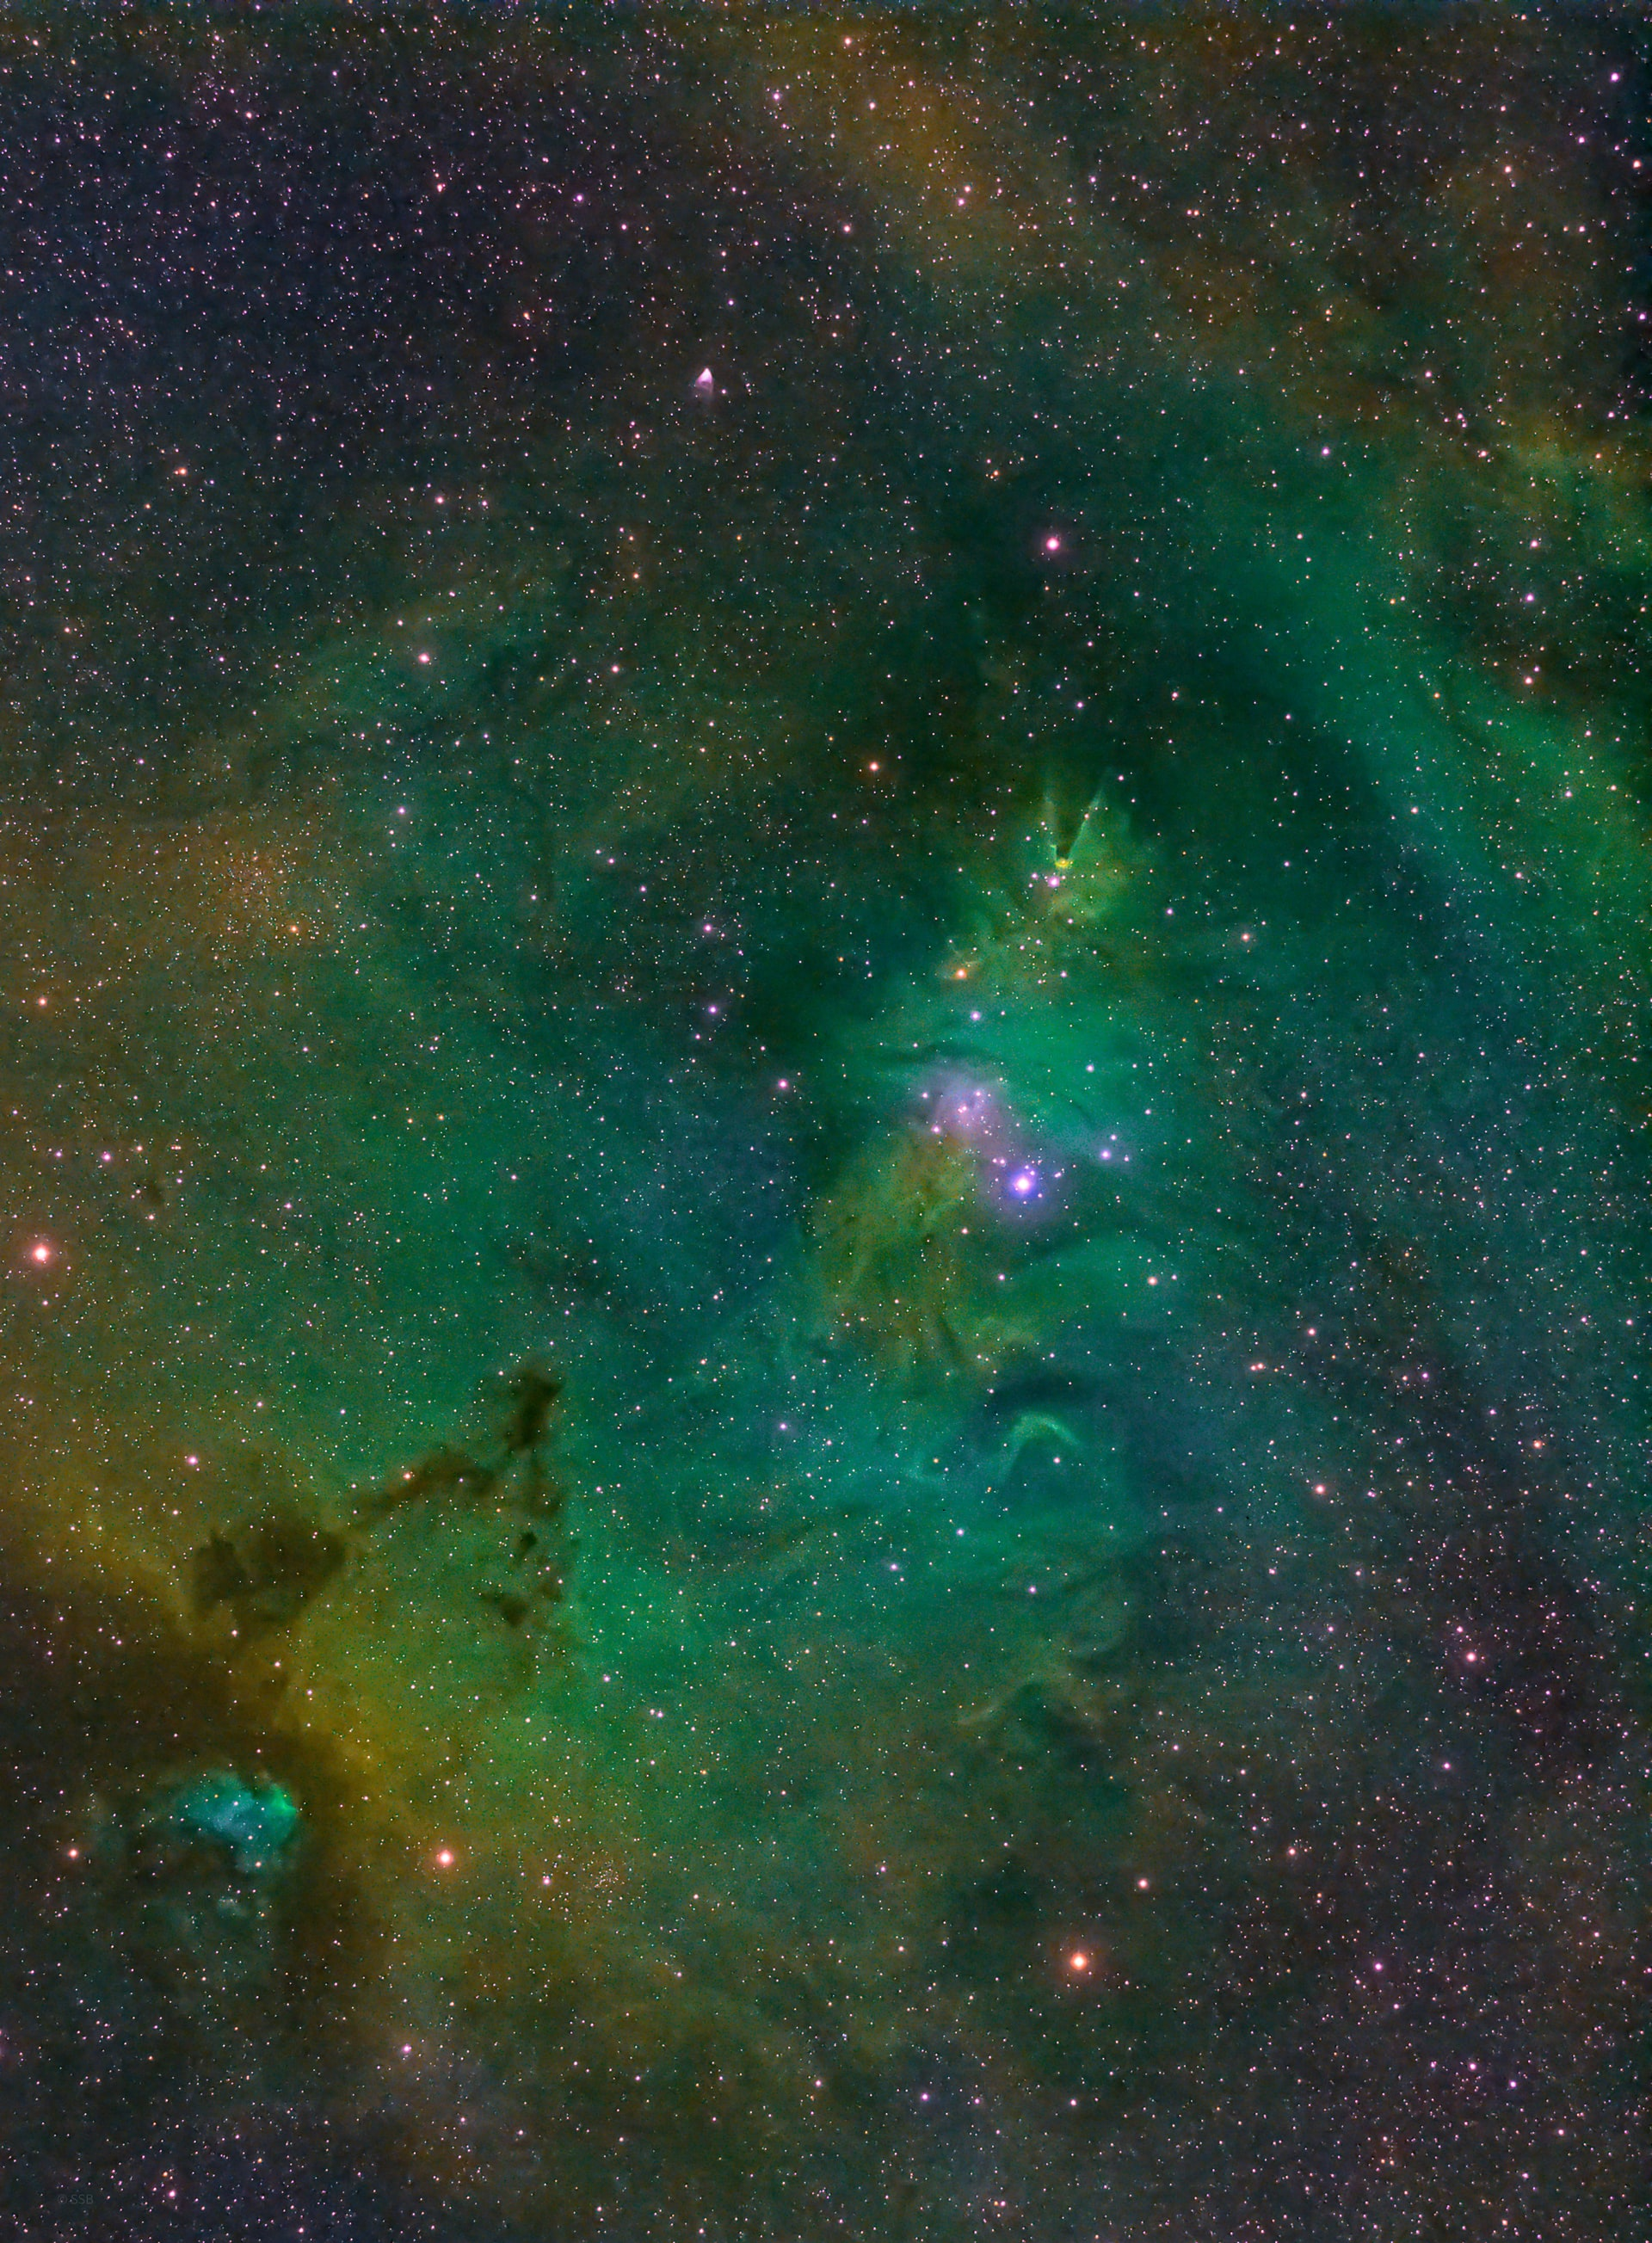
\includegraphics[width=\paperwidth]{./img/aldebaran.jpg}}
\begin{frame}
\huge{\textcolor{white}{\textbf{0x9: Buffer Overflows, Format Strings and Integer Bugs}}}
\end{frame}
}

\section{0xA: Architectural Attacks}
{
\usebackgroundtemplate{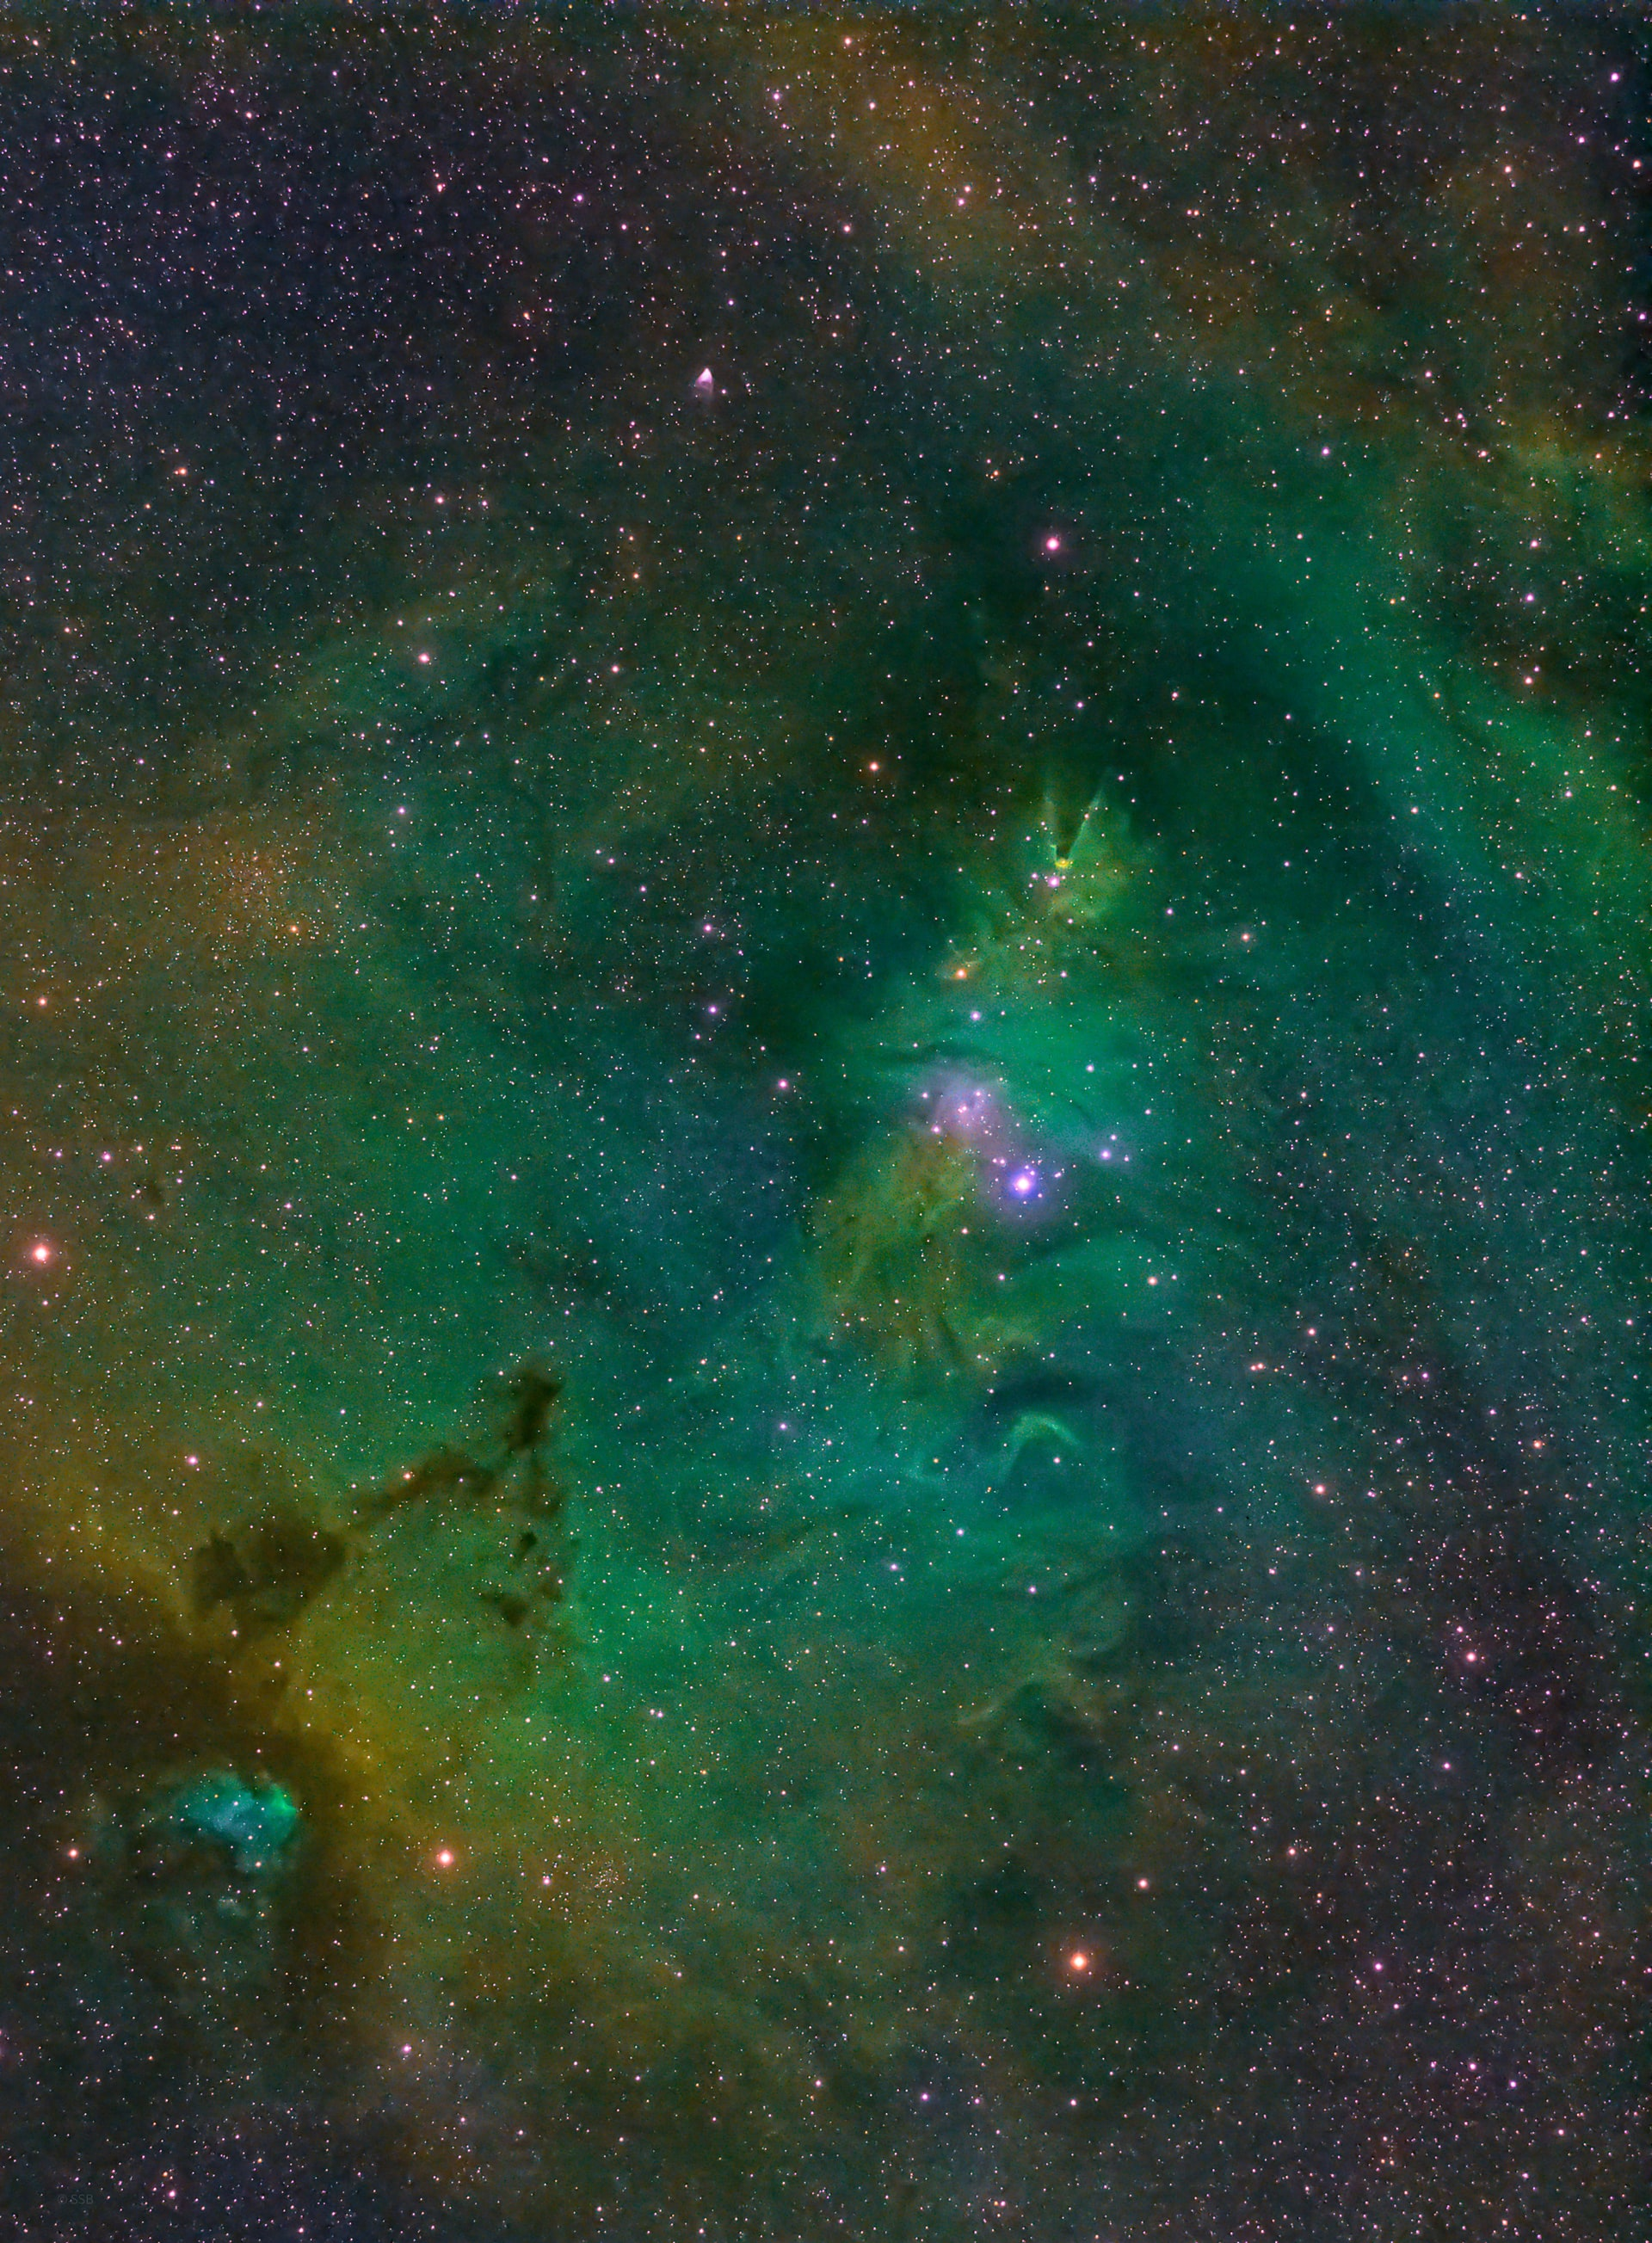
\includegraphics[width=\paperwidth]{./img/aldebaran.jpg}}
\begin{frame}
\huge{\textcolor{white}{\textbf{0xA: Architectural Attacks}}}
\end{frame}
}

\section{0xB: Attacks on the Web Server}
{
\usebackgroundtemplate{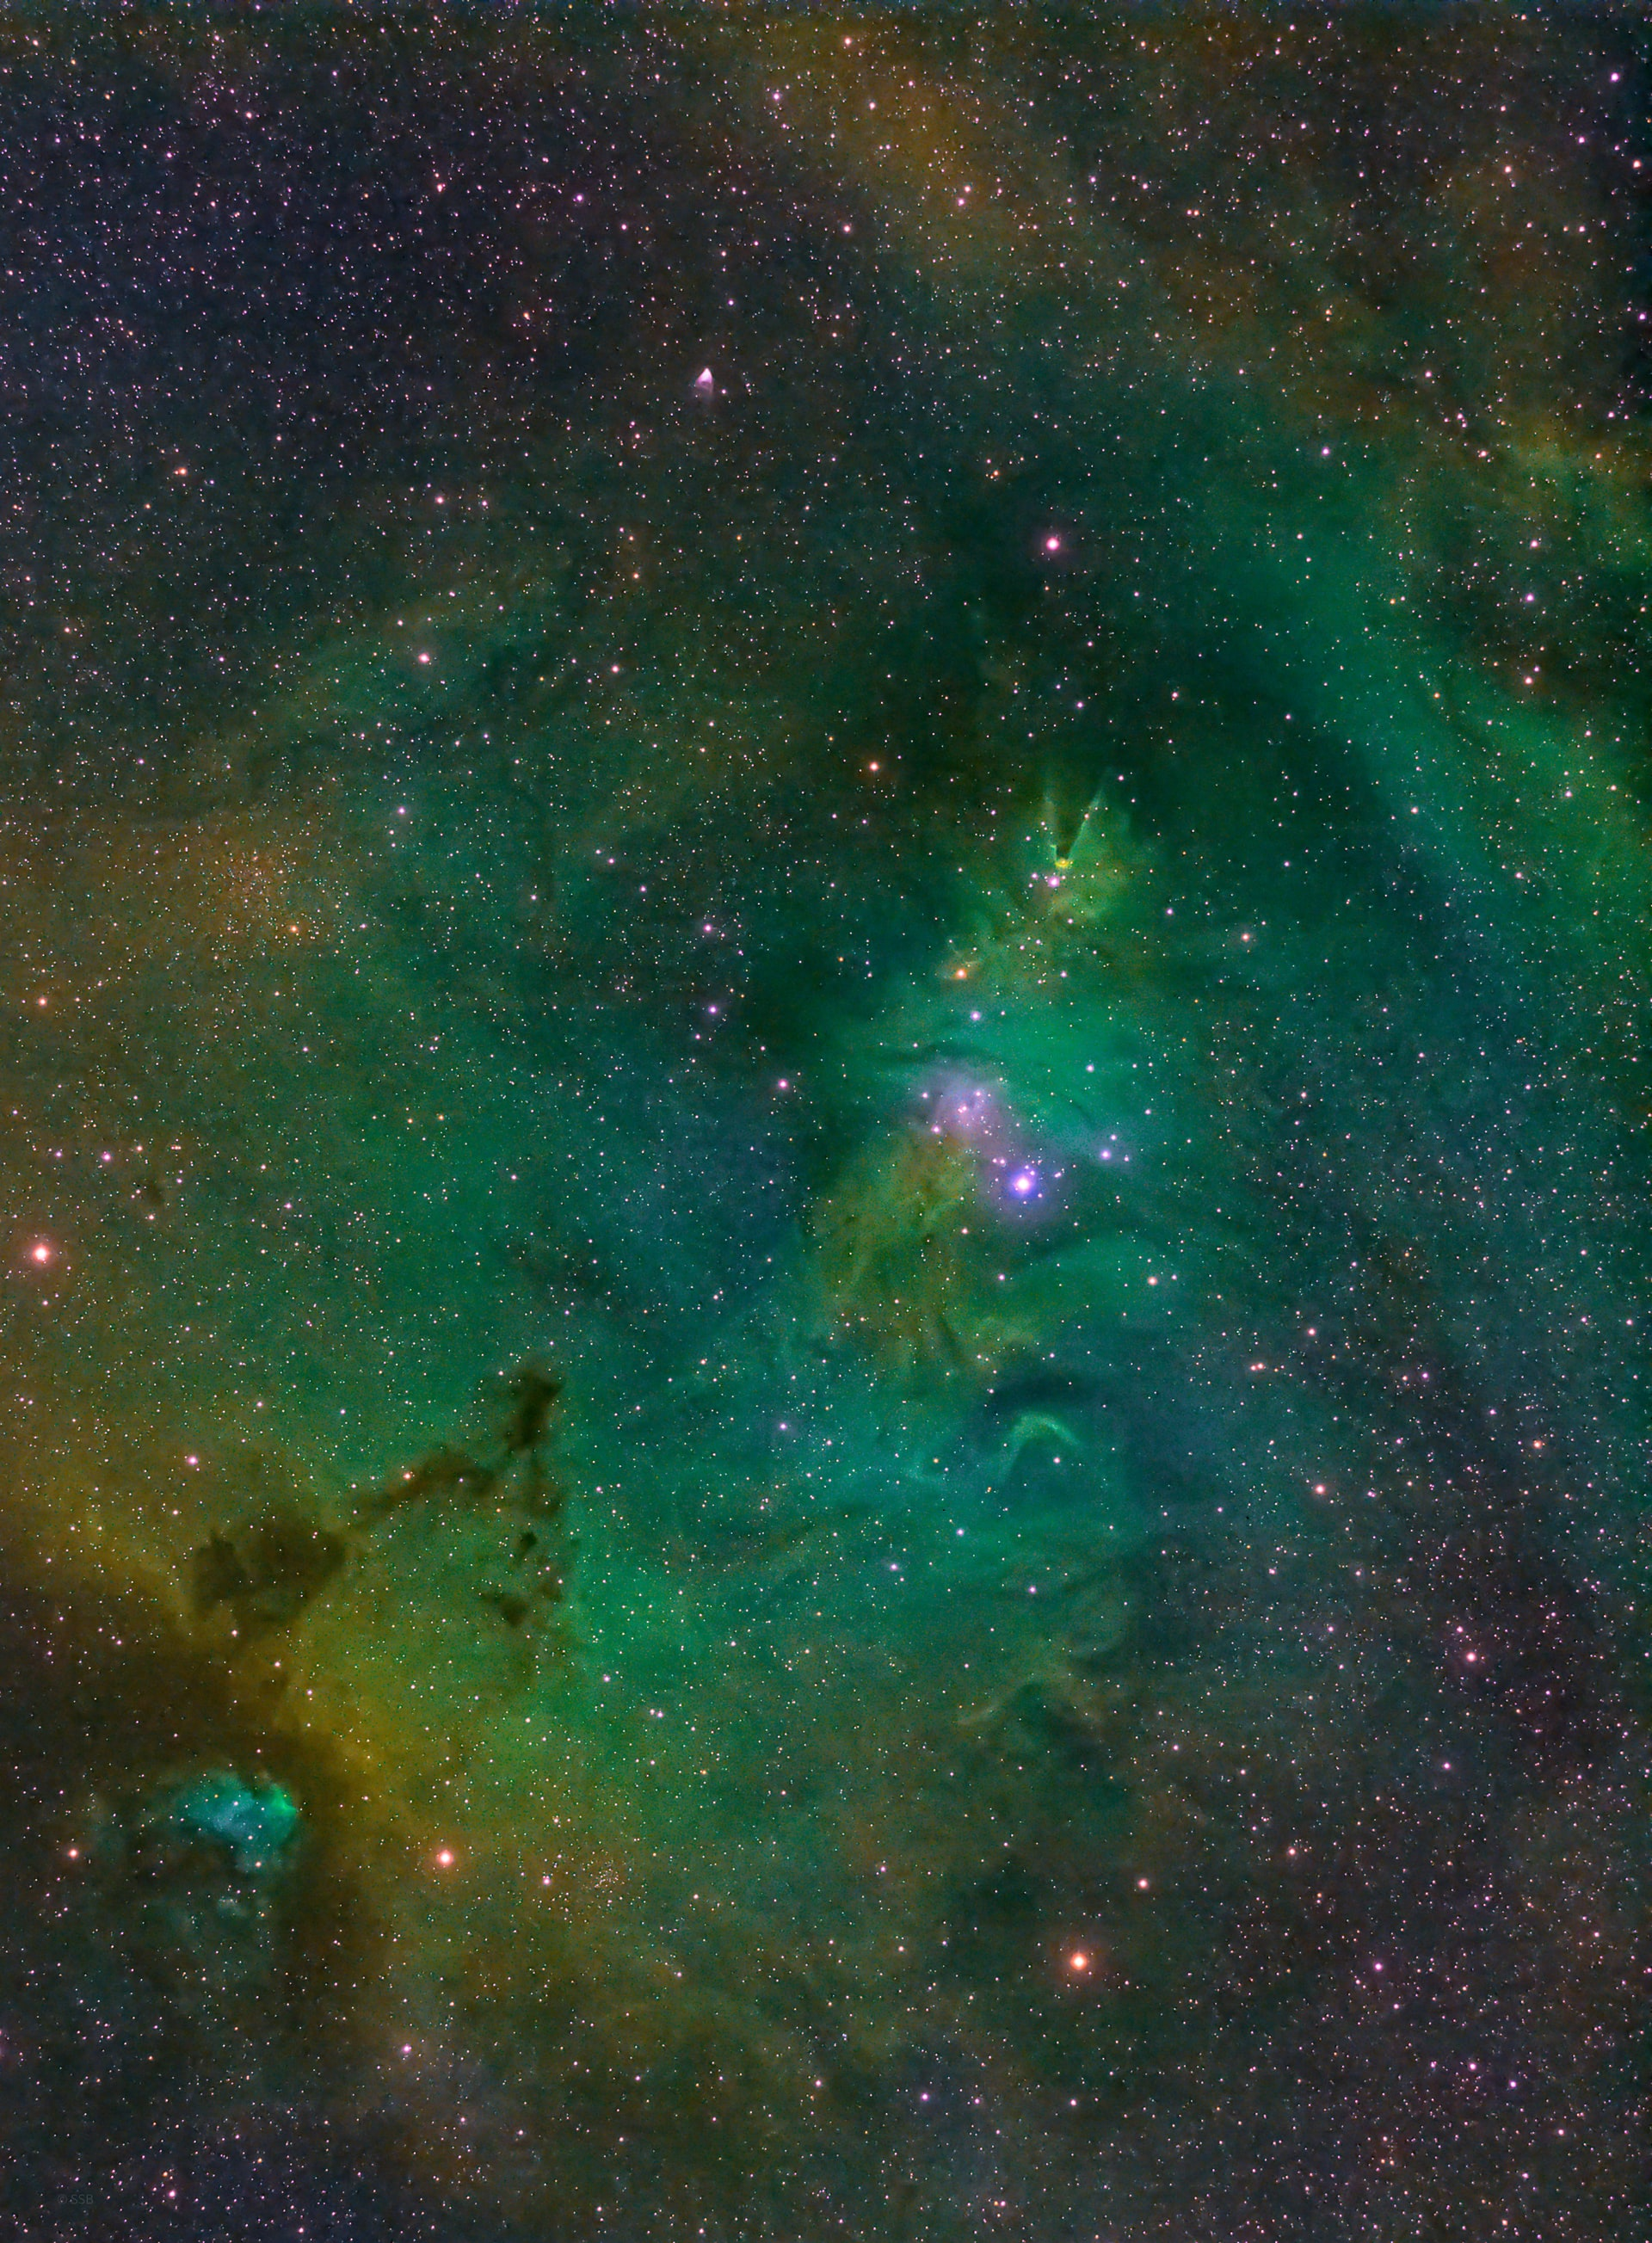
\includegraphics[width=\paperwidth]{./img/aldebaran.jpg}}
\begin{frame}
\huge{\textcolor{white}{\textbf{0xB: Attacks on the Web Server}}}
\end{frame}
}


{
\usebackgroundtemplate{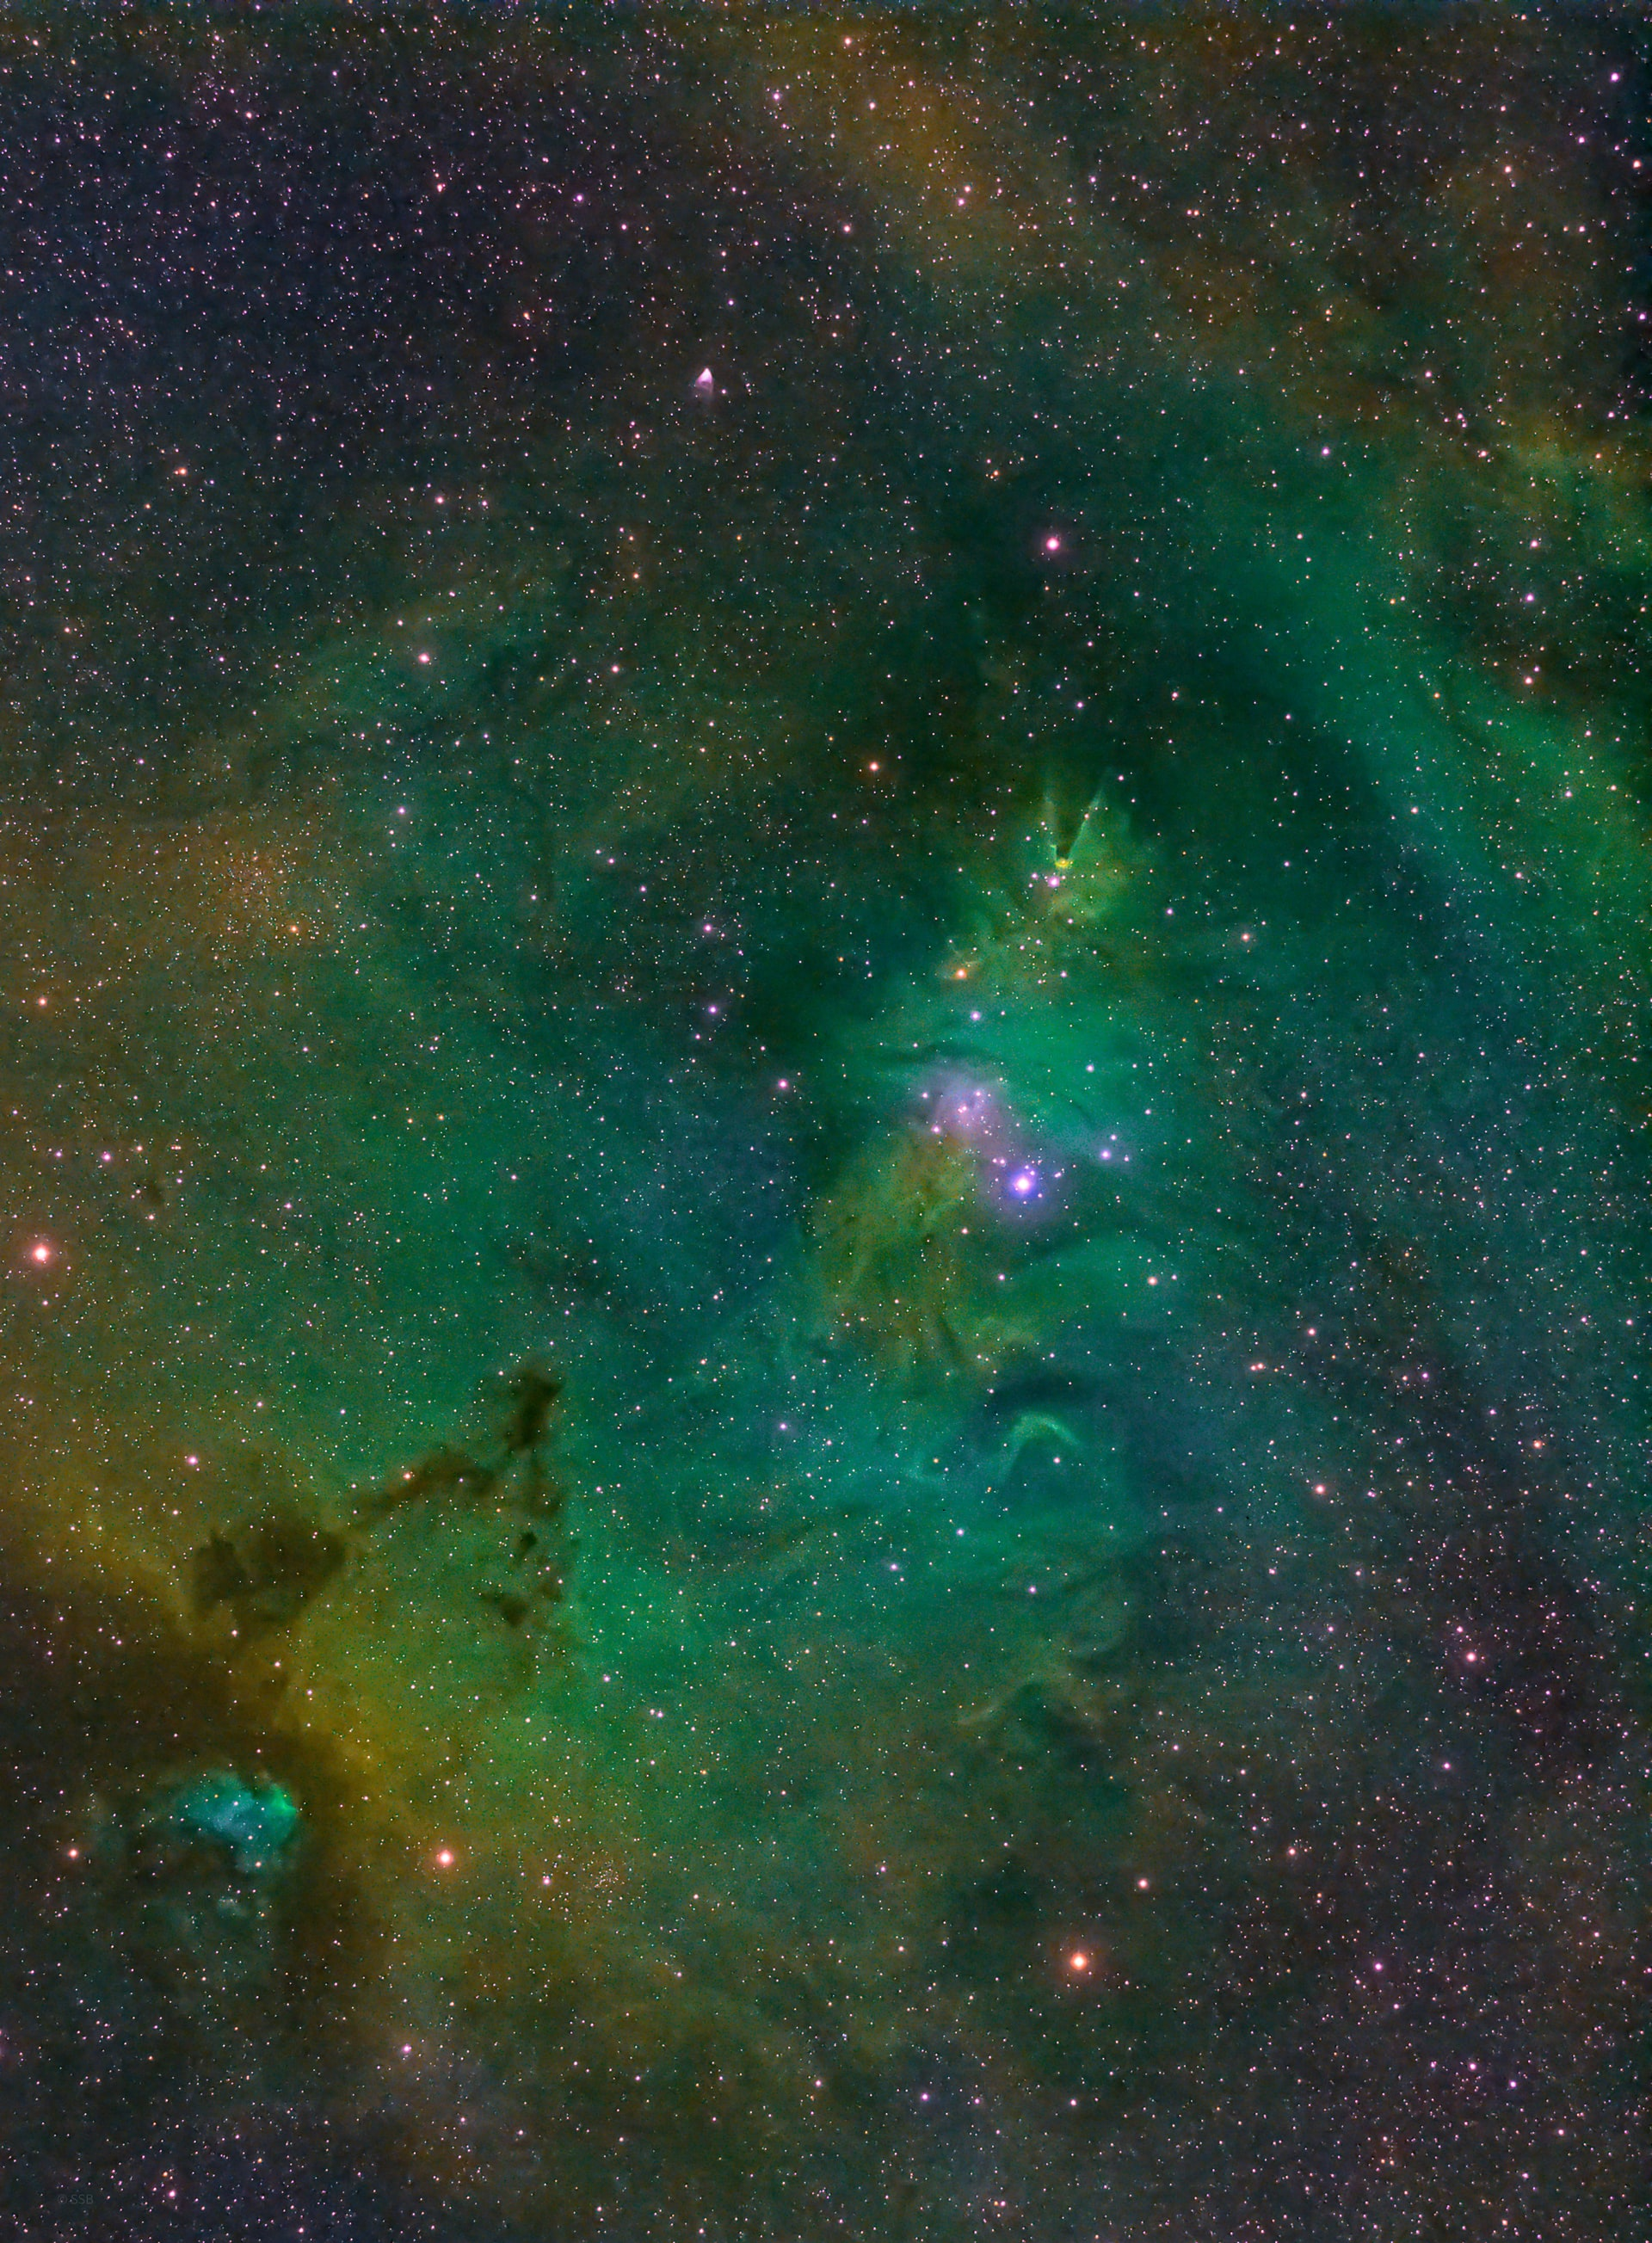
\includegraphics[width=\paperwidth]{./img/aldebaran.jpg}}
\begin{frame}
\huge{\textcolor{white}{\textbf{0xC: Misc}}}
\end{frame}
}

\begin{frame}
    \frametitle{More Things to Consider}
    One \pause
    Two \pause
    Three
\end{frame}

\begin{frame}
    \frametitle{Bibliography}

\end{frame}

\bibliographystyle{plain}
\bibliography{ref/bibliography}

\end{document}